%\documentclass[conference, oribibl]{IEEEtran}
\documentclass[runningheads,a4paper,oribibl]{llncs}
\usepackage{llncsdoc}

% *** MISC UTILITY PACKAGES ***
%
\usepackage{amssymb}
\usepackage{verbatim}
\setcounter{tocdepth}{3}
\usepackage{adjustbox,lipsum}

\usepackage{graphicx}
\graphicspath{ {Figs/} }

\usepackage{amsmath}
\usepackage{multirow}
\usepackage{slashbox}
\usepackage{amsfonts}

\usepackage{algpseudocode}
\usepackage{algorithm}
\usepackage{epstopdf}
\usepackage{array}
\usepackage{enumerate}

\usepackage{epstopdf}

\usepackage{url}
%\urldef{\mailsa}\path|{khanhtv, mizuhito}@jaist.ac.jp|    

%ieee requirements
%\usepackage[utf8]{inputenc}
%\usepackage[T1]{fontenc}
%\usepackage{microtype} 
%\usepackage{balance}

%user definitions
\newcommand{\Nat}{{\mathbb N}}
\newcommand{\Real}{{\mathbb R}}
\newcommand{\Rat}{{\mathbb Q}}
\newcommand{\suppress}[1]{} % Comment out text.
\newcommand{\mizuhito}[1]{\{{\bf Mizuhito:~\sf #1}\}} % Highlight text.
\newcommand{\khanh}[1]{\{{\bf Khanh:~\sf #1}\}} % Highlight text.

\newcommand{\smallHead}[1]{%
    \par\vspace{.35cm}\noindent\textbf{#1}%
    \par\noindent\ignorespaces%
}

\newcommand\TTTT{%
 \textsf{T\kern-0.2em\raisebox{-0.3em}T\kern-0.2emT\kern-0.2em\raisebox{-0.3em}2}%
}

% correct bad hyphenation here
\hyphenation{op-tical net-works semi-conduc-tor}


\begin{document}
%
% paper title
% can use linebreaks \\ within to get better formatting as desired
% Do not put math or special symbols in the title.
\title{{\bf raSAT}: SMT Solver for Polynomial Inequality}

\author{Vu Xuan Tung\inst{1}, To Van Khanh\inst{2}, and Mizuhito Ogawa\inst{1}} 
\institute{
Japan Advanced Institute of Science and Technology\\
\email{\{tungvx,mizuhito\}@jaist.ac.jp}
\and 
University of Engineering and Technology, Vietnam National 
University, Hanoi \\
\email{khanhtv@vnu.edu.vn}
}

\tableofcontents

% make the title area
\maketitle

% As a general rule, do not put math, special symbols or citations
% in the abstract
\begin{abstract}
This paper presents an SMT (Satisfiability Modulo Theory) solver {\bf raSAT} for polynomial inequality. 
It consists of a simple iterative approximation refinement, called {\bf raSAT} loop, 
which is an extension of the standard ICP (Interval Constraint Propagation) with testing. 
Two approximation schemes consist of interval arithmetic (over-approximation) and 
testing (under-approximation), to accelerate SAT detection. 
If both fails, input intervals are refined by decomposition. 

ICP is robust for large degrees, but the number of boxes (products of intervals) to explore 
exponentially explodes with respect to the number of variables. 
We design strategies for boosting SAT detection on the choice of a variable to decompose
and a box to explore. 

Several heuristic measures, called {\em SAT likelihood}, {\em sensitivity}, and the number of 
unsolved atomic polynomial constraints, are compared on Zankl and Meti-tarski benchmarks from 
QF\_NRA category of SMT-LIB. They are also evaluated by comparing {\bf Z3 4.3}, \textbf{dReal-2.15.01} and {\bf iSAT3}. 
raSAT loop is extended with the use of the Intermediate Value Theorem to solve equality. This extension is evaluated on equalities of Zankl, Meti-tarski and Keymaera families.
We also show a simple modification to handle mixed integers, and experiments on 
AProVE benchmark from QF\_NIA category of SMT-LIB. 
\end{abstract}
% no keywords
%\keywords{interval arithmetic, affine arithmetic, SMT, polynomial constraints, 
%testing, abstract DPLL.}


% For peer review papers, you can put extra information on the cover
% page as needed:
% \ifCLASSOPTIONpeerreview
% \begin{center} \bfseries EDICS Category: 3-BBND \end{center}
% \fi
%
% For peerreview papers, this IEEEtran command inserts a page break and
% creates the second title. It will be ignored for other modes.
% \IEEEpeerreviewmaketitle

\section{Introduction}
{\em Polynomial Constraint solving} over real (integer) numbers is to find an assignment from real (integer) numbers to variables 
that satisfies given polynomial inequality/equality. 
%For instance, $\exists x y. -y^2 + (x^2 - 1) y - 1 > 0 \wedge -x^2 - y^2 + 4 > 0$ is 
%such an example. This is an easy formula, but proving its satisfiability and 
%showing a satisfiable instance (e.g., $x = 1.8$, $y=0.9$) are not so easy.  
%its satisfiability and a satisfiable instance 
%(e.g., $x = 1.8$, $y=0.9$) are not so easy.  		
%
Many applications are reduced to solving polynomial constraints, such as 
\begin{itemize}
\item {\bf Locating roundoff and overflow errors}, 
which is our motivation~\cite{Ngoc:2009:ORE:1685167.1685421,Ngoc:2010:CRE:1858996.1859056}. 
%DSP decoders in practice are defined by reference algorithms in C using floating point arithmetic. 
%In embedded systems, often it is replaced with fixed point arithmetic, 
%which may cause visible noises. 
%and locating such roundoff error source is not easy. 
%For instance, consider DSP decoder like mpeg4. Usually, the decoder definition is given by a reference 
%algorithm in C, which uses floating point number. 
%In an embedded system, it is tempting to replace floating 
%point into fixed point numbers. However, naive replacement would cause 

\item {\bf Automatic termination proving}, 
which reduces termination detection to finding a suitable ordering~\cite{Lucas:2008:CCS:1361735.1361760}, 
e.g., \TTTT~\footnote{\url{http://cl-informatik.uibk.ac.at/software/ttt2/}}, 
AProVE~\footnote{\url{http://aprove.informatik.rwth-aachen.de}}. 
%as a solution of polynomial constraints. 

\item {\bf Loop invariant generation}. 
Farkas's lemma is a popular approach in linear loop invariant generation~\cite{Colon}, 
and is reduced to degree $2$ polynomials. 
%matrix multiplications. 
%degree $2$ polynomial constraints. 
%Farkas's lemma uses products of matrices, and it requires solving polynomial constraints of degree 2.
Non-linear loop invariant~\cite{Sankaranarayanan:2004:NLI:982962.964028} requires more complex polynomials.

\item {\bf Hybrid system}. SMT solvers for polynomial constraints over real numbers (QF\_NRA) are often used as backend engines~\cite{Sankaranarayanan04constructinginvariants}. 

\item {\bf Mechanical contrnol design}. 
Proportional-integral-derivative controllers are simple but widely used, and designing parameters is 
reduced to polynomial constraints~\cite{control}. 
%Fujitsu used polynomial constraints solving to design PID control of HDD head movement
\end{itemize}	

Solving polynomial constraints on real numbers is decidable~\cite{tarski}, 
though that on integers is undecidable ({\em Hilbert's 10th problem}). 
Quantifier elimination by cylindrical algebraic decomposition (QE-CAD)~\cite{qecad} 
is a well known technique, and 
implemented in Mathematica, Maple/SynRac, Reduce/Redlog, QEPCAD-B, and recently 
in some SMT solvers~\cite{Jovanovic13}. 
It can solve general formula at the cost of DEXPTIME, which hardly work up to 8 variables and degree 10.
Satisfiability targets on an existential problem, and 
{\em Variant quantifier elimination}~\cite{Hong2012883} reduces polynomial constraint solving to 
polynomial optimization problems, which are solved by Groebner basis in EXPTIME. 

A practical alternative is Interval Constraint Propagation ({\em ICP}), 
which are used in SMT solver community, e.g., {\bf iSAT3}~\cite{isat}, 
{\bf dReal}~\cite{dRealCADE13}, and \textbf{RSolver}~\cite{rsolver}. 
ICP is based on over-approximation by interval arithmetics, and iteratively refines by
interval decompositions. 
It is practically often more efficient than algebraic computation 
with weaker theoretical completeness. 
\begin{comment}
For polynomial inequality 
$\exists x_1 \in (a_1,b_1) \cdots x_n \in (a_n,b_n) . \wedge_{i} f_i > 0$, 
\begin{itemize}
\item If $\exists x_1 \in (a_1,b_1) \cdots x_n \in (a_n,b_n) . \wedge_{i} f_i > 0$ is SAT, 
ICP eventually detects it. 
\item If $\exists x_1 \in [a_1,b_1] \cdots x_n \in [a_n,b_n] . \wedge_{i} f_i \geq 0$ is UNSAT, 
ICP eventually detects it
\end{itemize}
under the assumptions of bounded intervals. 
\begin{figure}[ht]
%\begin{minipage}[b]{1.0\linewidth}
\centering
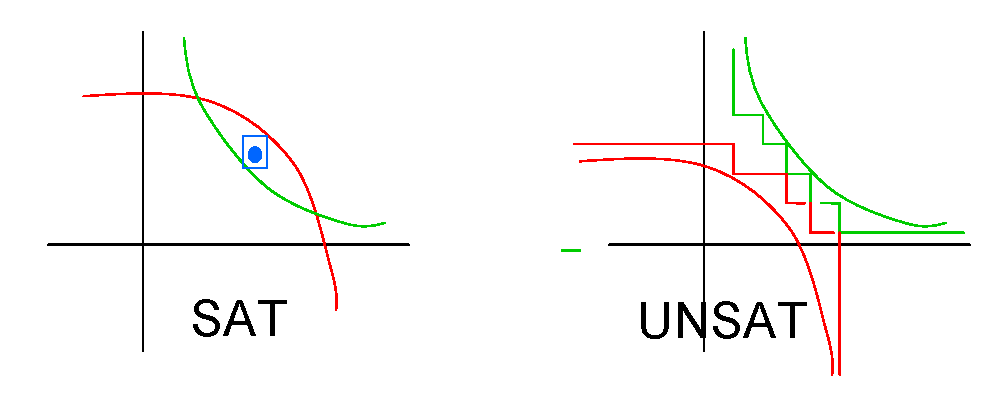
\includegraphics[height=1.2in,width=3.4in]{FigCompleteness.eps} 
\caption{SAT and UNSAT detection by ICP} 
\label{fig:complete} 
%\end{minipage}
\end{figure} 

The boundary part is reduced to polynomial equality checking, 
which would be solved by using algebraic methods, like Groebner basis. 
Alternatively, by loosening equality to $\delta$-equality, 
$\delta$-completeness is obtained~\cite{dRealCADE13}. 
\end{comment}

This paper presents an SMT solver {\bf raSAT} for polynomial inequality. 
It consists of a simple iterative approximation refinement, called {\bf raSAT} {\em loop}, 
which is an extension of the standard ICP with testing to accelerate SAT detection. 
Two approximation schemes consist of interval arithmetic (over-approximation) and 
testing (under-approximation), to accelerate SAT detection. 
If both fails, input intervals are refined by decomposition. 
%
Compared to typical ICP solvers, {\bf raSAT} 
\begin{itemize}
\item introduces testing (as an under-approximation) to accelerate SAT detection, 
\item applies various interval arithmetic, e.g., Affine intervals~\cite{Messine_extensionsof,Ngoc:2009:ORE:1685167.1685421,VanKhanh201227}, 
which enables to analyze the effects of input values, and 
\item SAT confirmation step by an error-bound guaranteed floating point package {\bf iRRAM}\footnote{% 
\tt http://irram.uni-trier.de}, to avoid soundess bugs caused by roundoff errors. 
\end{itemize}
This design is more on SAT detection oriented, since from our preliminary experiences, 
if the target problems have several hundred variables, solvable cases in practice are 
either SAT or UNSAT with small UNSAT core. 
Thus, acceleration of SAT detection and finding UNSAT core will be keys for scalability. 

As \textbf{iSAT3}, \textbf{raSAT} applies outward rounding~\cite{Hickey:2001:IAP:502102.502106} in Interval arithmetics to avoid soundless bugs due to round-off error of floating arithmetic operations. As a consequence, answers of raSAT (SAT or UNSAT) (SAT instances found in testing is verified by \textbf{iRRAM}) are guaranteed to be sound.

ICP is robust for larger degrees, but the number of boxes (products of intervals) to explore 
exponentially explodes when variables increase. 
Thus, design of strategies for selecting variables to decompose and boxes to explore is crucial 
for efficiency. Our strategy design is, 
\begin{itemize}
\item a box with more possiblity to be SAT is selected to explore, which is estimated by 
several heuristic measures, called {\em SAT likelihood}, 
and the number of unsolved atomic polynomial constraints, and
\item a more influential variable is selected for multiple test cases and decomposition, 
which is estimated by {\em sensitivity}. 
\end{itemize} 
Note that {\em SAT likelihood} and {\em sensitivity} are estimated using interval arithmetic. 
Especially, the latter can be applied only with Affine intervals. 
{\bf raSAT} also applies incremental search, which is often faster in practice. 
\begin{itemize}
\item {\bf Incremental widening}. 
Starting {\bf raSAT} loop with a smaller interval, and if it is UNSAT, enlarge the input intervals
and restart. 
\item {\bf Incremental deepening}. 
Starting with the bound that each interval will be decomposed no smaller than it. 
If neither SAT nor UNSAT is detected, take a smaller bound and restart. 
\end{itemize} 
Efficient UNSAT core % with error bound guaranteed floating point arithmetic 
is left for future work. 

They are compared on Zankl and Meti-Tarski benchmarks from 
QF\_NRA category of SMT-LIB\footnote{\tt http://www.smtlib.org/}. 
They are also evaluated by comparing 
{\bf Z3 4.3}\footnote{\tt http://z3.codeplex.com} and {\bf iSAT3}. 
Another advantage of {\bf raSAT} is the ease to handle mixed intergers, 
and experiments on AProVE benchmark from QF\_NIA category of SMT-LIB compares {\bf raSAT} with 
{\bf Z3 4.3}. 
Although {\bf Z3 4.3} performs the best, {\bf raSAT} shows comparable SAT detection on 
very large problems (e.g., with several hundred variables) with the combination of 
{\em SAT likelihood} and {\em sensitivity}. 


\subsection*{Related Work} \label{sec:relate}

Non-linear constraints are still under development, and SMT solvers adapt 
several approachs other than ICP. 

\medskip \noindent
\textbf{QE-CAD}. ~RAHD \cite{Passmore09combineddecision} and 
Z3 4.3 (which is referred as nlsat in~\cite{Jovanovic13}) include QE-CAD. 
%such as QEPCAD-B, Reduce/Redlog, and Mathematica. 
QE-CAD is precise and detects beyond SAT instances (e.g., SAT regions), 
scalability is still challenging, since it is DEXPTIME. 
%Since QE-CAD is DEXPTIME wrt the number of variables, 

\medskip \noindent
\textbf{Virtual substitution (VS)}. ~
%Virtual substitution is an EXPTIME algorithm 
%applicable when the degree of each variable does not exceed 4. 
SMT-RAT toolbox \cite{smtrat}\cite{vssmt} combines 
VS, incremental DPLL, and %less lazy and 
eager theory propagation. 
Z3 (version 3.1), the winner of QF\_NRA in SMT competition 2011, 
combines VS, ICP, and linearization.

\medskip \noindent
\textbf{Bit-blasting}. ~Bid-blasting in bounded bit width is often used in SMTs for QF\_NIA. 
UCLID~\cite{Bryant07decidingbit-vector} reduces the number of bits (i.e., narrowing bounds for SAT instances) 
as an under-approximation, and removes clauses as an over-approximation. 
They refine each other, which shares a similar sprit with {\bf raSAT} loop. 
MiniSmt~\cite{Zankl:2010:SNR:1939141.1939168}, the winner of QF\_NRA in SMT competition 2010, 
applies it for rational numbers with symbolic representations for prefixed algebraic numbers. 
MiniSmt can show SAT quickly with small degree polynomials, but due to the bounded bit encoding, 
it cannot conclude UNSAT.
Bit-blasting also suffers a lot when the degree of polynomials increases. 

\medskip \noindent
\textbf{Linearization}. ~
Linearization of polynomials is often used over integers, such as Barcelogic~\cite{Borralleras:2009:SNP:1614530.1614561}, 
which substitutes all possible integers in a given-bound to an argument of a multiplication. 
Then, multiplications are reduced to an exhaustive search on linear constraints. 
CORD \cite{cordic} uses another linearization, called 
CORDIC (COrdinate Rotation DIgital Computer) for real numbers. 
Both Barcelogic and CORD apply Yices for solving linear constraints.
Linearization also suffers a lot when the degree of polynomials increases. 
%\mizuhito{Check CORD is whether bit-blasting or linearization}. 
Because \textbf{raSAT} in the same category of using ICP with \text{iSAT3} and \text{dReal}, next part is going to take a look at details of methodologies used in these solvers.
\subsection*{iSAT3}
Although \textbf{iSAT3} also uses Interval Arithmetic (IA), its algorithm integrates IA with DPLL procedure~\cite{dpll} tighter than that of \textbf{raSAT}. During DPLL procedure, in addition to an assignment of literals, \textbf{iSAT3} also prepares a data structure to store interval boxes where each box corresponds to one decision level of DPLL procedure's assignment. In \textbf{UnitPropagation} rule, intead of using standard rule, \textbf{iSAT3} searches for clauses that have all but one atoms being inconsistence with the current interval box. When some atom are selected for the literals assignment, this tool tries to use the selected atoms to contract the corresponding box to make it smaller. In order to do this, \textbf{iSAT3} convert each inequality/equation in the given constraints into the conjunction of the atoms of the following form by introducing additional variables:
\begin{center}
\begin{tabular}{l c l}
atom &::=& bound $\mid$ equation \\
bound &::=& variable relation rational\_constant \\
relation &::=& $< \mid \le \mid = \mid \ge \mid >$ \\
equation &::=& variable = variable bop variable \\
bop &::=& $+ \mid - \mid \times$
\end{tabular}
\end{center}
In other words, the resulting atoms are of the form, e.g., either $x > 10$ or $x = y + z$. For example, the constraint \[x^2 + y^2 < 1\]
is converted into:
\[\left\{ 
  \begin{array}{l}
    x_1 = x^2\\
    x_2 = y^2\\
    x_3 = x_1 + x_2\\
    x_3 < 1
   \end{array}
    \right.\]
From the atoms of these form, the contraction can be easily done for interval boxes:
\begin{itemize}
\item[$\bullet$] For the bound atom of the form, e.g., $x > 10$, if the bound is $x \in \langle 0, 100 \rangle$, then the contracted box contain $x \in \langle 10, 100 \rangle$.
\item[$\bullet$] For the equations of three variables $x = y \text{ bop } z$, from bounds of any two variables, we can infer the bound for the remaining one. For example, from
\[\left\{ 
  \begin{array}{l}
    x = y.z\\
    x \in \langle 1, 10 \rangle \\
    y \in \langle 3, 7 \rangle\\
   \end{array}
    \right.\]
we can infer that \[z \in \langle \frac{1}{7}, \frac{10}{3} \rangle \]
\end{itemize}
When the \textbf{UnitPropagation} and contraction can not be done, \textbf{iSAT3} split one interval (decomposition) in the current box and select one decomposed interval to explore which corresponds to \textbf{decide} step. If the contraction yields an empty box, a conflict is detected and the complement of the bound selection in the last split needs to be asserted. This is done via \textbf{learn} the causes of the conflict and \textbf{backjump} to the previous bound selection of the last bound selection. In order to reason about causes of a conflict, \textbf{iSAT3} maintains an implication graph to represents which atoms lead to the asserting of one atom. 
\subsection*{dReal}
In stead of showing satisfiability/unsatisfiability of the polynomial constraints $\varphi$ over the real numbers, \textbf{dReal} proves that either
\begin{itemize}
\item [$\bullet$] $\varphi$ is unsatisfiable, or 
\item [$\bullet$] $\varphi^\delta$ is satisfiable. 
\end{itemize}
Here, $\varphi^\delta$ is the $\delta$-weakening of $\varphi$. For instance, the $\delta$-weakening of $x = 0$ is $|x| \le \delta$. Any constraint with operators in $\{<, \le, > , \ge, =, \not=\}$ can be converted into constraints that contains only $=$ by the following transformations.
\begin{itemize}
\item [$\bullet$] \textbf{Removing $\not=$}: Each formula of the form $f \not= 0$ is transformed into $f > 0 \vee f < 0$.
\item [$\bullet$] \textbf{Removing $<$ and $\le$}: Each formula of the form $f < 0$ or $f \le 0$ is transformed into $-f \ge 0$ or $-f > 0$ respectively.
\item [$\bullet$] \textbf{Removing $>$ and $\ge$}: Each formula of the form $f > 0$ or $f \ge 0$ is transformed into $f - x = 0$ by introducing an auxiliary variable $x$ that has bound $[0, m]$ or $(0, m]$ respectively. Here, $m$ is any rational number which is greater than the maximum of $f$ over intervals of variables. As the result, \textbf{dReal} requires the input that ranges of variables must be compact.
\end{itemize}

Note that the satisfiability of $\varphi^\delta$ does not imply that of $\varphi$. \textbf{dReal}'s methodology~\cite{Gao:2012:9DP:2352896.2352921} also cooperates DPLL with ICP in the lazy manner as in \textbf{raSAT}.

\medskip 
%{\bf raSAT} applies SAT confirmation to avoid soundness errors caused by roundoff/overflow errors. 
%Another static analysis based approach is found in~\cite{SilvaTACAS12}. 



\section{Over and Under Approximation Theories and Their Refinement}
\label{sec:raSATloop} 
\subsection{Approximation Theory}

Let 
$F = \exists x_1 \in I_1 \cdots x_n \in I_n. \bigwedge \limits_j \psi_j(x_1,\cdots,x_n)$, 
%\exists x_1 \ldots x_n. (\underbrace{\bigwedge \limits_i x_i \in I_i}_{I}) \wedge 
%                       (\underbrace{\bigwedge \limits_j \psi_j(x_1,\cdots,x_n)}_{P})
where $\psi_j(x_1,\cdots,x_n)$ is an atomic formula of the form $p_j(x_1,...,x_n) \circ 0$ with $p_j(x_1,...,x_n)$ is a polynomial over variables $x_1,...,x_n$ and $\circ \in \{>, <\}$. 
%
$F$ is equivalnet to 
$\exists x_1 \ldots x_n. (\bigwedge \limits_i x_i \in I_i) \wedge (\bigwedge \limits_j \psi_j(x_1,\cdots,x_n))$, 
and we call $\bigwedge \limits_i x_i \in I_i$ {\em interval constraints}, and 
we refer $\bigwedge \limits_j \psi_j(x_1,\cdots,x_n)$ by $\psi(x_1,\cdots,x_n)$. 
Initially, interval constraints have a form of the conjunction $\bigwedge \limits_i x_i \in I_i$, 
and later by refinement, $x_i \in I_i$ is decomposed into a clause $\bigvee_k x_i \in I_{i_k}$, 
which makes a CNF. 

As an SMT (SAT modulo theory) problem, 
boolean variables are assigned to each $x_i \in I_{i_k}$, 
and truth assignments is produced by a SAT solver, 
which are proved or disproved by a background theory $T$ whether it satisfies $\psi(x_1,\cdots,x_n)$. 
\sloppy
As notational convention, $m$ (the lower case) denotes 
an assignment $\{x_i \mapsto r_i \mid i \in \{1, \cdots, n\}\}$ from real numbers $r_i$'s to $x_i$'s, and 
$M$ (the upper case) denotes a truth assignment on $x_i \in I_{i_k}$'s. 
We write $m \in M$ when for all $i \in \{1, \cdots, n\}$, we have $c_i \in I_{i_k}$ for all $x_i \in I_{i_k}$'s that are assigned true by $M$. 

We assume {\em very lazy theory learning}~\cite{dpll}, and 
a backend theory $T$ is applied only for a full truth assignment $M$. 
%We regard $M$ as a conjunction $\bigwedge \limits_i x_i \in I_{i_j}$. 
\begin{itemize}
\item If an instance $m$ satisfies $\psi(x_1,\cdots,x_n)$, we denote $m \models_T \psi(x_1,\cdots,x_n)$. 
\item If each instance $m$ with $m \in M$ satisfies $\psi(x_1,\cdots,x_n)$, 
we denote $M \models_T \psi(x_1,\cdots,x_n)$. 
\end{itemize}

\begin{definition} \label{def:app}
Let $F = \exists x_1 \in I_1 \cdots x_n \in I_n. \psi(x_1,\cdots,x_n)$. 
For a truth assignment on $M$, $F$ is 
\begin{itemize}
\item $T$-valid if $M \models_T \psi(x_1,\cdots,$ $x_n)$, 
\item $T$-satisfiable ($T$-SAT) if $m \models_T \psi(x_1,\cdots,x_n)$ 
for some $m \in M$, and 
\item $T$-unsatisfiable ($T$-UNSAT) if $M \models_T \neg \psi(x_1,\cdots,x_n)$. 
\end{itemize}
If $T$ is clear from the context, we simply say valid, satisfiable, and unsatisfiable. 
\end{definition}

%%%%%%%%%%%%%
\suppress{
Then, Fig. \ref{fig:T_result} illustrates Definition~\ref{def:app}. 
\begin{figure} [ht]
\centering
\begin{minipage}[b]{0.45\linewidth}
  \includegraphics[height=1.8in,width=1.9in]{T_result.eps}
\caption{Results of a target constraint $F$ in a theory $T$}
\label{fig:T_result}
\end{minipage}
\quad
\begin{minipage}[b]{0.45\linewidth}
   \includegraphics[height=2.2in,width=2.3in]{frame_app.eps}
\caption{{\bf raSAT} loop}
\label{fig:frame}
\end{minipage}
\end{figure}
}
%%%%%%%%%%%%%%%%%%%%%%%%%%%%%%%%

\begin{definition} \label{def:ApproxTheory}
Let $T, O.T, U.T$ be theories. 
\begin{itemize}
\item $O.T$ is an {\em over-approximation theory} (of $T$) 
if $O.T$-UNSAT implies $T$-UNSAT, and
\item $U.T$ is an {\em under-approximation theory} (of $T$)
if $U.T$-SAT implies $T$-SAT. 
\end{itemize}
We further assume that $O.T$-valid implies $T$-valid. 
\end{definition}

%Note that $O.T$-valid can be regarded as $U.T$, since $O.T$-valid implies $T$-valid, thus $T$-SAT. 
A typical ICP applies $O.T$ only as an interval arithmetic. 
Later in Section~\ref{sec:approximation}, we will instantiate interval arithmetic as $O.T$. 
Adding to $O.T$-valid, {\bf raSAT} introduce testing as $U.T$ to accelerate SAT detection. 



\subsection{Over-Approximation Theory Refinement}
\label{sec:soundness}

From now on, We focus on a \emph{polynomial inequality} such that 
$I_i$ and $\psi_j(x_1,\cdots,x_n)$ are an open interval $(a_i,b_i)$ and 
an atomic polynomial inequaltiy (API) $f_j > 0$, respectively. 
We denote $\mathbb{S}(f_j) = \{x \in \Real^n \mid f_j > 0 ~\text{holds}\}$.

For ICP, it is folklore that, for polynomial inequality 
$\exists x_1 \in (a_1,b_1) \cdots x_n \in (a_n,b_n) . \wedge_{j} f_j > 0$, 
\begin{itemize}
\item if $\exists x_1 \in (a_1,b_1) \cdots x_n \in (a_n,b_n) . \wedge_{j} f_j > 0$ is SAT, 
ICP eventually detects it, and 
\item if $\exists x_1 \in [a_1,b_1] \cdots x_n \in [a_n,b_n] . \wedge_{j} f_j \geq 0$ is UNSAT, 
ICP eventually detects it, 
\end{itemize}
under the assumptions of fair decomposition and bounded intervals $(a_i,b_i)$ for all $i \in \{1, \cdots, n\}$. 
We will prepare terminology and briefly review this fact. 

%%%%%%%%%%%%%%%%%%%%%%
\suppress{
\begin{definition} \label{def:poly}
A polynomial inequality is a bounded quantification 
$\exists x_1 \in I_1 \cdots x_n \in I_n. \psi(x_1,\cdots,x_n)$ 
such that 
\begin{itemize}
\item each $I_i$ is an open interval $x_i \in (a_i,b_i)$, and 
\item $\psi(x_1,\cdots,x_n)$ is a conjunction of $f_j > 0$ 
where $f_j$ is a polynomial over $\{x_1, \cdots, x_n\}$. 
\end{itemize}
$f_i > 0$ is called an atomic polynomial inequality (API). 
We denote $\mathbb{S}(F) = \{x \in \Real^n \mid F ~\text{holds}\}$.
\end{definition}

\begin{example} \label{examp:poly_ieq}
$\exists x \in (-1,3)~y \in (2,4) . (x^3y - y^4 > 0) \wedge (y^3 -xy >0)$
is an example of a polynomial inequality with 2 variables and 2 APIs. 
\end{example}
}
%%%%%%%%%%%%%%%%%%%%%%

\begin{definition}
An \emph{open box} of dimension $n$ is a set $(a_1,b_1) \times \cdots \times (a_n,b_n)$ 
where $a_i, b_i \in \Real, a_i \leq b_i$.  
For $\mathfrak{a} = (a_1, \cdots, a_n)$ and $\mathfrak{b} = (b_1, \cdots, b_n)$, 
we denote $(a_1,b_1) \times \cdots \times (a_n,b_n)$ by $(\mathfrak{a}, \mathfrak{b})$. 
\end{definition}

The set of all open boxes is a basis of Euclidean topology on $\Real^n$. 
In $\Real^n$, a set $U$ is compact if, and only if, $U$ is a bounded closed set. 
We denote a closure of a set $U$ by $\overline{U}$. 
%
Since a polynomial is continuous, 
$\mathbb{S}(\bigwedge \limits_{j=1}^m f_j > 0)$ is an open set. 
Note that $\Rat$ is dense in $\Real$, and an SAT instance in reals can be replaced with one in rationals. 

%%%%%%%%%%%%%%%%%%%%%%%%%%%%%%
\suppress{
\begin{lemma} \label{cor:rattoreal}
For a polynomial inequality
$F = \exists x_1 \in I_1 \cdots x_n \in I_n. \bigwedge \limits_{j=1}^m f_j > 0$, 
If there exists an SAT instance of F in $\Real^n$, there exists also in $\Rat^n$. 
\end{lemma}

\begin{lemma} \label{cor:refinement}
Suppose that $a_j < b_j$ for $1 \leq j \leq n$ and $f_i$'s are polynomials. 
Assume $a_k < c < b_k$ for some $k$. 
Then, 
$\exists x_1 \in (a_1,b_1) \cdots x_n \in (a_n,b_n). \bigwedge \limits_{i=1}^m f_i > 0$ 
is SAT (resp. UNSAT) if, and only if, 
$\exists x_1 \in (a_1,b_1) \cdots x_k \in (a_k,c) \cdots x_n \in (a_n,b_n). 
 \bigwedge \limits_{i=1}^m f_i > 0 
 \vee 
 \exists x_1 \in (a_1,b_1) \cdots x_k \in (c,b_k) \cdots x_n \in (a_n,b_n)). 
 \bigwedge \limits_{i=1}^m f_i > 0$ 
is SAT (resp. UNSAT). 
\end{lemma}

\begin{pf}
We show for the SAT case. If-part is obvious. For only-if-part, 
since $\mathbb{S}(\bigwedge \limits_{i=1}^m f_i > 0)$ is an open set, 
if $y \in (a_1,b_1) \times \cdots \{c\} \cdots \times (a_n,b_n)$ satisfies 
$\bigwedge \limits_{i=1}^m f_i > 0$, 
there exists $x_1 \in (a_1,b_1) \cdots x_k \in (a_k,c) \cdots x_n \in (a_n,b_n)$
(also $x_1 \in (a_1,b_1) \cdots x_k \in (c,b_k) \cdots x_n \in (a_n,b_n)$) that satisfies
$\bigwedge \limits_{i=1}^m f_i > 0$. 
\end{pf}

Lemma~\ref{cor:rattoreal} says that proving SAT of $F$ in $\Real$ is reduced to 
that in $\Rat$. 
Lemma~\ref{cor:refinement} says that, in the refinement step, we can apply refinement 
$x_k \in (a_k,b_k)$ to $x_k \in (a_k,c) \vee x_k \in (c,b_k)$, 
instead of $x_k \in (a_k,c] \vee x_k \in (c,b_k) $
(i.e., $c$ is ignored). 
}
%%%%%%%%%%%%%%%%%%%%%%%%%%%%%%

Initially, interval constraints consists of conjunction only. Later, by refinements, it becomes a CNF. 


\begin{example} \label{examp:poly_ieq}
$\exists x \in (-1,3)~y \in (2,4) . (x^3y - y^4 > 0) \wedge (y^3 -xy >0)$
is an example of a polynomial inequality with 2 variables and 2 APIs. 

For instance, $x \in (-1,3)$ and $y \in (2,4)$ are refined to smaller intervals
such that 
$\exists x \in (-1,1) y \in (2,4) . (x^3y - y^4 > 0) \wedge (y^3 -xy >0) \vee 
 \exists x \in (1,3) y \in (2,4) . (x^3y - y^4 > 0) \wedge (y^3 -xy >0)$, 
which results a CNF 
$(x \in (-1,1) \vee x \in (1,3)) \wedge (y \in (2,4)) \wedge (x^3y - y^4 > 0) \wedge (y^3 -xy >0)$.
%(only the CNF formula $(x \in (-1,1) \vee x \in (1,3)) \wedge (y \in (2,4))$ is given to SAT solver).
%\mizuhito{could you fulfill? Direct encoding seems a DNF?}. 
\end{example}

Note that an interval arithmetic used in ICP is a converging theory. 

\begin{definition} \label{def:completeOT}
Let
$F = \exists x_1 \in I_1 \cdots x_n \in I_n. \bigwedge \limits_{j=1}^m f_j > 0$
be a polynomial inequality such that each $I_i$ is bounded. 
An over-approximation theory $O.T$ is {\em converging} 
if, for each $\delta > 0$ and $c = (c_1, \cdots, c_n) \in I_1 \times \cdots \times I_n$, 
there exists $\gamma > 0$ such that 
$\bigwedge \limits_{i=1}^n x_i \in (c_i - \gamma, c_i + \gamma) \models_{O.T} 
 \bigwedge \limits_{j=1}^m (f_j(c) - \delta < f_j(x) < f_j(c) + \delta)$. 
\end{definition}

$O.T$ refinemnet loop is shown in Fig.~\ref{fig:OTrefine}~(a). 
A standard ICP based algorithm of an SMT solver applies it with $O.T$ as a classical interval arithemtic. 
The variation of interval arithemtic will be presented in Section~\ref{sec:approximation}. 
\begin{figure}[ht]
\begin{minipage}[b]{1.0\linewidth}
\centering
\begin{tabular}{c@{\qquad}c}
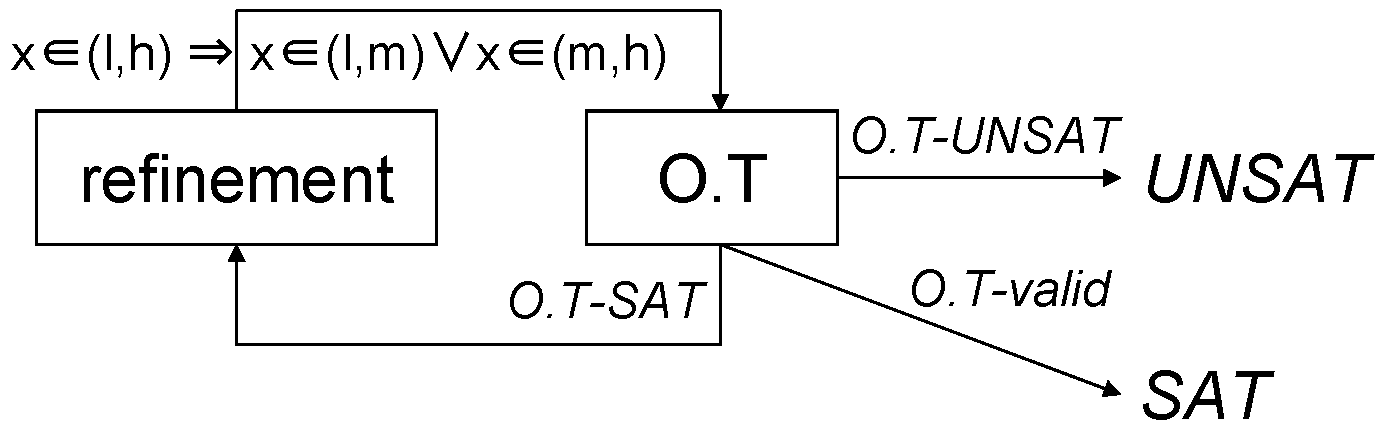
\includegraphics[height=0.6in,width=1.7in]{OTloop.png} & 
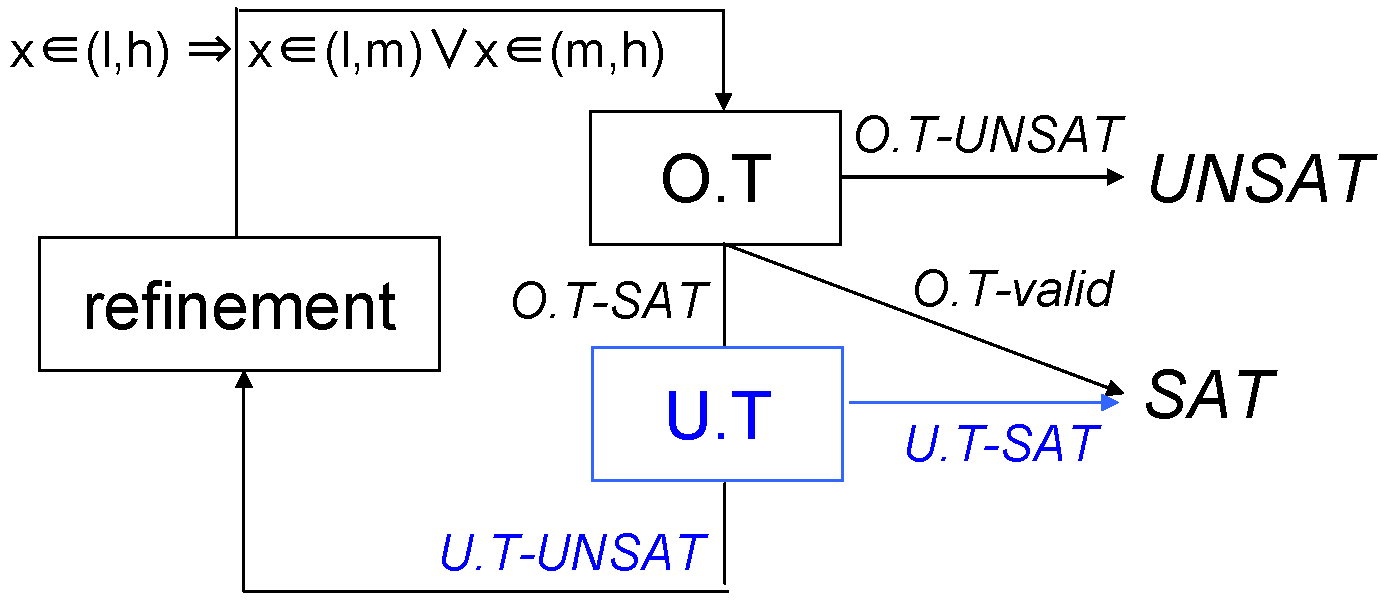
\includegraphics[height=0.9in,width=1.7in]{rasatloop.png} \\   
\mbox{(a) $O.T$ refinement loop} & \mbox{{\bf raSAT} loop} \\
\end{tabular}
\end{minipage} 
\caption{Rfinement loops} 
\label{fig:OTrefine} 
\end{figure}


\begin{definition} 
Let
$F = \exists x_1 \in I_1 \cdots x_n \in I_n. \bigwedge \limits_{j=1}^m f_j > 0$
for $I_i = (a_i,b_i)$.
A refinement strategy is {\em fair}, if, for each $c_i \in (a_i,b_i)$ and $\gamma > 0$, 
a decomposition of $I_i$ for each $i$ eventually occurs in $(c_i - \gamma, c_i + \gamma)$ 
(as long as neither SAT nor UNSAT is detected). 
\end{definition}

\begin{theorem} \label{th:RelComp}
Let
$F = \exists x_1 \in I_1 \cdots x_n \in I_n. \bigwedge \limits_{j=1}^m f_j > 0$
for $I_i = (a_i,b_i)$.
Assume that an over-approximation theory $O.T$ is converging, 
each $(a_i,b_i)$ is bounded, and a refinement strategy is fair. 
Then, 
\begin{itemize}
\item if $\exists x_1 \in (a_1,b_1) \cdots x_n \in (a_n,b_n) . \wedge_{j} f_j > 0$ is SAT, 
$O.T$ refinement loop eventually detects it, and
\item if $\exists x_1 \in [a_1,b_1] \cdots x_n \in [a_n,b_n] . \wedge_{j} f_j \geq 0$ is UNSAT, 
$O.T$ refinement loop eventually detects it.  
\end{itemize}
\end{theorem}


\begin{proof} 
The former is proved by the fact that, if $F$ is SAT, there exists a non-empty neiborhood (open box) 
in $\cap~\mathbb{S}(f_j)$. 
If the box decomposition strategy is fair, the refinemnet will eventually find such an open box. 

For the latter, assume that 
$\overline{F} = \exists x_1 \in [a_1,b_1] \cdots x_n \in [a_n,b_n] . \wedge_{j} f_j \geq 0$ is UNSAT. 
Thus, $\cap~\overline{\mathbb{S}(f_j)} = \emptyset$. 
Let $\delta_{j,k} = min \{|f_j(\bar{x}) - f_k(\bar{x})| \mid \bar{x} \in I_1 \times \cdots \times I_n\}$. 
Since $f_i$'s are continuous and $\overline{I_i}$'s are compact, $\delta_{j,k}$ is well defined,
and $\delta_{j.k} > 0$ for some $j,k$. 
Let $\delta = \frac{min \{ \delta_{j,k} \}}{2}$. 
Since $O.T$ is converging, there exists $\gamma > 0$ for $\delta > 0$ 
satisfying Definition~\ref{def:completeOT}, and fair decomposition eventually finds open boxes
such that $\mathbb{S}(f_j)$ and $\mathbb{S}(f_k)$ are separated. 
\qed
\end{proof}

Limitations for detecting UNSAT occur on \emph{kissing} and \emph{convergent} cases. 
Fig.~\ref{fig:limit} left shows a kissing case 
$x^2 + y^2 < 2^2 \wedge (x-4)^2 + (y-3)^2 < 3^2$ such that 
$\overline{\mathbb{S}(- x^2 - y^2 + 2^2)} \cap \overline{\mathbb{S}(- (x-4)^2 - (y-3)^2 + 3^2)} 
= \{(x,y) \mid (1.6, 1.2)\}$. 
Thus, there are no coverings to separate them. 
%$x^2 + y^2 < 2^2$ and $(x-4)^2 + (y-3)^2 < 3^2$. 
%
Fig. \ref{fig:limit} right shows a convergent case 
$y > x + \frac{1}{x} \wedge y < x \wedge x > 0$, which is equivalent to 
$xy > x^2 + x \wedge y < x \wedge x > 0$. 
%The open box is $(0,\infty) \times (0,\infty)$ and 
There are no finite coverings to separate them. 
%$y > x + \frac{1}{x}$ and $y < x$ for $x > 0$. 

\begin{figure}[ht]
%\begin{minipage}[b]{1.0\linewidth}
\centering
\begin{tabular}{cc}
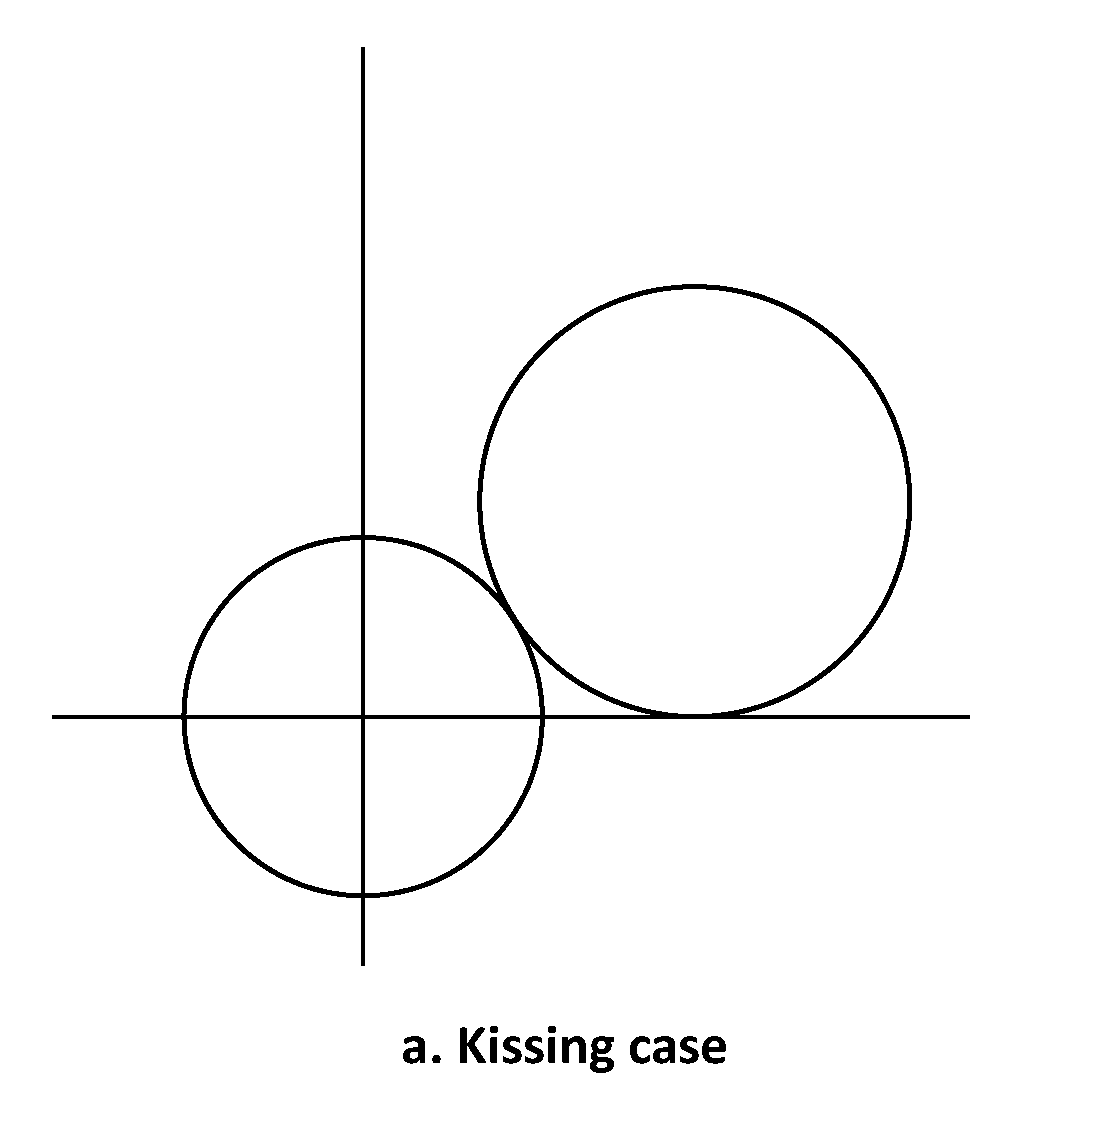
\includegraphics[height=1.65in,width=1.7in]{kissing.eps} &
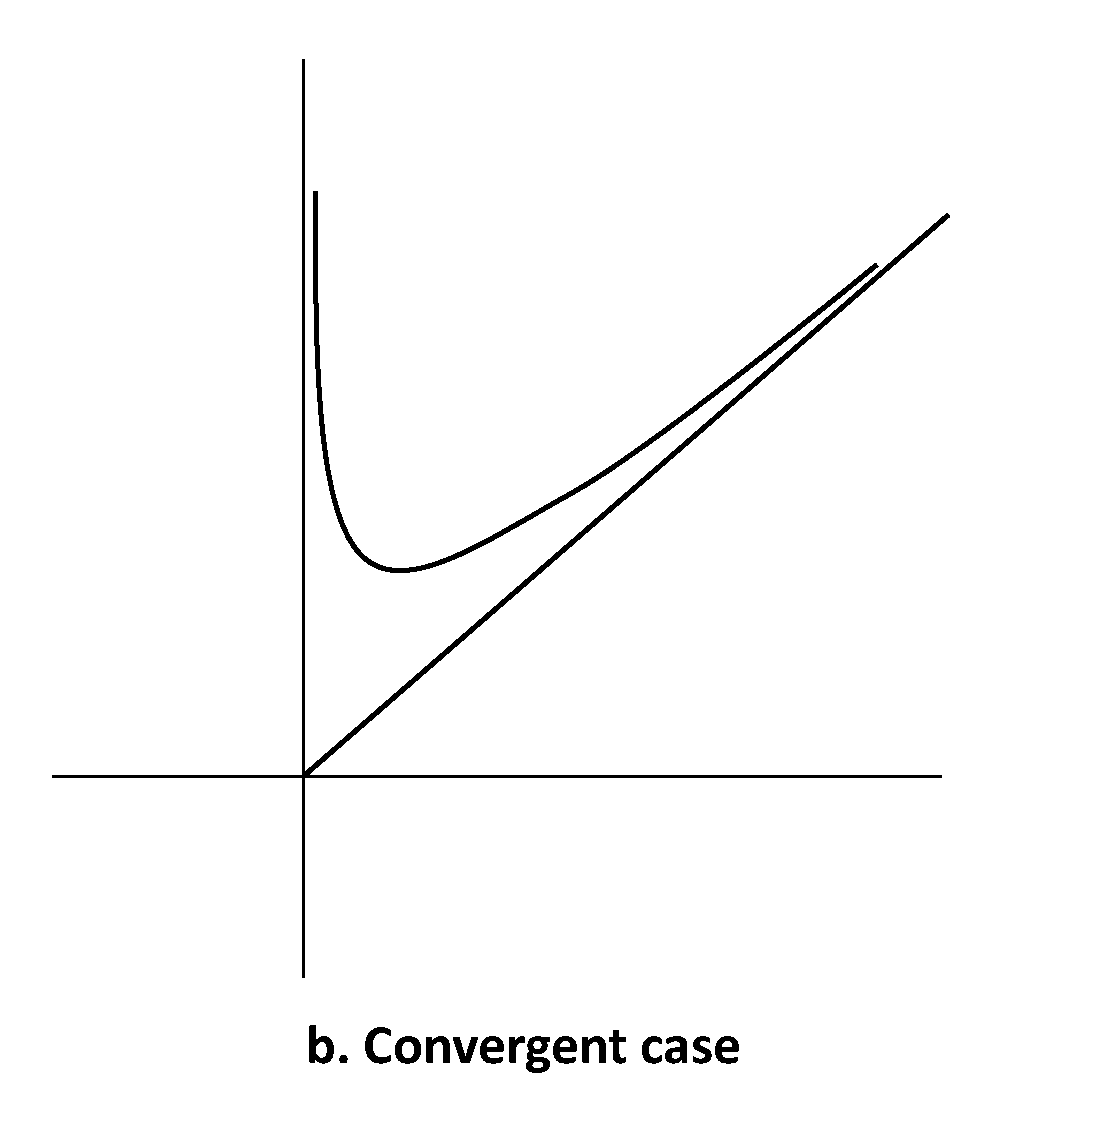
\includegraphics[height=1.65in,width=1.7in]{convergence.eps}
\end{tabular}
\caption{Limitations for proving UNSAT} 
\label{fig:limit} 
%\end{minipage}
\end{figure} 



\subsection{raSAT loop}

Although an $O.T$ refinement loop is enough to implement an ICP based SMT solver, 
we extend it as {\bf raSAT} (SAT by refinement of approximations) loop to accelerate SAT detection 
by adding $U.T$, which works as in Fig.~\ref{fig:OTrefine}~(b). 
\begin{enumerate}
\item When an over-approximation theory $O.T$ detects $O.T$-UNSAT (resp. $O.T$-valid), 
answer UNSAT (resp. SAT). 
\item When an under-approximation theory $U.T$ detects $U.T$-SAT, answer SAT. 
\item If neither holds, a refinement is applied. 
\end{enumerate}

Our design of an SMT solver {\bf raSAT} applies two heuristic features. 
\begin{itemize}
\item Incremental widening intervals, and incremental deeping search 
(Section~\ref{sec:incsearch}). 
\item 
Heurstic measures {\em SAT-likelihood} and {\em sensitivity}, 
for selection of a variable to decompose and a box to explore. 
(Section~\ref{sec:SATheuristics}). 
\end{itemize} 

{\bf raSAT} also prepares various interval arithmetics as $O.T$ as in Section~\ref{sec:approximation}, 
whereas currently only random tesing (\emph{k-random ticks}, 
which consists of periodical $k$-test instances with a random offset) is prepared as $U.T$. 


\section{Interval arithmetic} \label{sec:approximation}

A typical theory for $O.T$ and $U.T$ are an interval arithmetic and testing, respectively. 
We say {\em IA-valid}, {\em IA-SAT}, and {\em IA-UNSAT}, when it is $O.T$-valid, $O.T$-SAT, and 
$O.T$-UNSAT, respectively. 
Similarly, we say {\em test-SAT} when it is $U.T$-SAT and {\em test-UNSAT} when $U.T$-UNSAT. 
Note that either IA-valid or test-SAT implies SAT, and IA-UNSAT implies UNSAT, 
whereas IA-SAT and test-UNSAT can conclude neither. 


%We instantiate testing to $U.T$ in Section~\ref{sec:raSATloop}. 
%%%%%%%%%%%%%%%%
\suppress{
\begin{definition}\label{def:testing}
%For $\exists x_1 \in (a_1,b_1) \cdots x_n \in (a_n,b_n). \bigwedge \limits_{i=1}^m f_i(x_1,\cdots,x_n) > 0$, 
Let $M = \bigwedge \limits_{i=1}^m x_i \in (a_i,b_i)$ and 
${\mathcal P} = \bigwedge \limits_{i=1}^m f_i(x_1,\cdots,x_n) > 0$. 
%
Let a choice function $\theta : (\Real \times \Real)^n \rightarrow \Real^n$ 
such that $\theta(M) \in (a_1,b_1) \times \cdots \times (a_n,b_n)$. 
Testing is a finite set $\Theta$ of choice functions. Then, we say 
\begin{itemize}
\item ${\mathcal P}$ is \emph{Test-SAT} under $M$ if $\theta(M)$ holds ${\mathcal P}$ 
for some $\theta \in \Theta$, and 
\item ${\mathcal P}$ is \emph{Test-UNSAT} under $M$ if $\theta(M)$ never holds ${\mathcal P}$ 
for each $\theta \in \Theta$. 
\end{itemize} 
%We denote $I \models_{test(\theta)} P$ if $\bigwedge \limits_{i=1}^m f_i(\theta(I)) > 0$ holds.
\end{definition}
}
%%%%%%%%%%%%%%%%


{\bf raSAT} prepares various Affine intervals, adding to classical interval (CI)~\cite{moore}, 
which keep lower and upper bounds. The weakness of CI is loss of dependency 
among values. For instance, $x - x$ is evaluated to $(-2,2)$ for $x \in (2,4)$. 

Affine Interval~\cite{Comba93affinearithmetic, Stolfi97self-validatednumerical} introduces \emph{noise symbols} $\epsilon$, 
which are interpreted as values in $(-1,1)$. 
For instance, $x = 3 + \epsilon$ describes $x \in (2,4)$, and 
$x - x = (3 + \epsilon) - (3 + \epsilon)$ is evaluated to $0$. 
The drawback is that the multiplication without dependency might be less precise than CI.
Affine intervals also cannot represent infinite intervals, e.g., $(0,\infty)$, 
since it becomes $\infty + \infty~\epsilon$. 
Forms of affine intervals vary by choices how to approximate multiplications. They are,
\begin{enumerate}[(i)]
\item $\epsilon \epsilon'$ is replaced with a fresh noise symbol 
($AF$)~\cite{Comba93affinearithmetic, Stolfi97self-validatednumerical}, 
\item $\epsilon \epsilon'$ is reduced to the fixed error noise symbol 
$\epsilon_{\pm}$ ($AF_1$ and $AF_2$) \cite{Messine_extensionsof},
\item $\epsilon \epsilon'$ is replaced with $(-1,1) \epsilon$ 
(or $(-1,1) \epsilon'$) ($EAI$)~\cite{Ngoc:2009:ORE:1685167.1685421},
\item $\epsilon \epsilon$ is reduced to fixed noise symbols 
$\epsilon_+$ or $\epsilon_{-}$ ($AF_2$) \cite{Messine_extensionsof}, 
\item Chebyshev approximation of $x^2$ introduces a noise symbol $|\epsilon|$ 
as an absolute value of $\epsilon$ with 
$\epsilon \epsilon = |\epsilon| |\epsilon| = |\epsilon| + (-\frac{1}{4}, 0)$ and
$\epsilon |\epsilon| = \epsilon + (-\frac{1}{4}, \frac{1}{4})$ \cite{VanKhanh201227}. 
%(Fig.~\ref{fig:chevabs}). 
%\item keeping products of noise symbols up to degree $2$ ($\epsilon_i \epsilon_j$),
\end{enumerate} 

%%%%%%%%%%%%%%%%%
\suppress{
\begin{remark}
For Affine intervals, \emph{sensitivity}~\cite{ngocsefm} of a variable
is a possible range of the absolute value of the coefficient of its corresponding $\epsilon$. 

%In Example~\ref{examp:sensitivity}, $CAI$ estimates the coefficient of $|\epsilon_1|$ as $\textbf{3}$, 
%which has the largest sensitivity and indicates $x$ the most influencial. 

Note that Affine interval works only for bounded intervals. 
For instance, $\infty + \infty \epsilon$ represents $(-\infty,\infty)$, which says nothing. 
Narrowing intervals as an incremental search (Section~\ref{sec:incsearch}) partilly depends on this fact. 
That is, if $\pm \infty$ is contained in an interval, first give finite upper/lower bounds and search 
within these bounds using an Affine interval. If UNSAT is concluded, then enlarge to the whole intervals 
using CI. 
\end{remark}
}
%%%%%%%%%%%%%%%%%


\begin{example} \label{examp:sensitivity}
Let $f = x^3 - 2xy$ with $x = (0,2)$ ($x = 1 + \epsilon_1$) and $y=(1,3)$ ($y = 2+\epsilon_2$), 
we have,
\begin{itemize}
\item $AF_2$ estimates the range of $f$ as 
$-3 - \epsilon_1 - 2\epsilon_2 + 3\epsilon_+ + 3\epsilon_{\pm}$, thus $(-9,6)$,
\item $CAI$ estimates the range of $f$ as 
$(-4,-\frac{11}{4}) + (-\frac{1}{4}, 0)\epsilon_1 - 2\epsilon_2 + \textbf{3}|\epsilon_1| + (-2,2)\epsilon_{\pm}$, 
thus $(-8,4.5)$.
\end{itemize}
\end{example}


%%%%%%%%%%%%%%%%%%%%%%%%%%
\suppress{
\begin{figure}[ht]
\begin{minipage}[b]{1.0\linewidth}
\centering
\begin{tabular}{ll}
\includegraphics[height=1.6in,width=1.7in]{chev1.pdf} &
\includegraphics[height=1.6in,width=1.7in]{chev2.pdf}
\end{tabular}
\caption{Chebyshev approximation of $x^2$ and $x~|x|$}
\label{fig:chevabs}
\end{minipage}
\end{figure}

$CAI$ \cite{tapas12} consists of (ii) and (v), which keeps better precision than iv)
for multiplicatins of the same variables, e.g., Taylor expansion. 
%To improve precision in estimating upper and lower bounds of polynomials, we apply 
%\textbf{Affine Arithmetic} such as $AF_1$, $AF_2$ \cite{af}, $CAI$ ~\cite{tapas12} 
%instead of Classical Interval \cite{moore}. 
%Note that upper and lower bounds estimated by IA are over-approximation bounds of polynomials.

}
%%%%%%%%%%%%%%%%%%%%%%%%%%
\suppress{
\begin{definition}
%For $\exists x_1 \in (a_1,b_1) \cdots x_n \in (a_n,b_n). \bigwedge \limits_{i=1}^m f_i(x_1,\cdots,x_n) > 0$, 
Let $M = \bigwedge \limits_{i=1}^m x_i \in (a_i,b_i)$ and 
${\mathcal P} = \bigwedge \limits_{i=1}^m f_i(x_1,\cdots,x_n) > 0$. 
%
Let $\delta_i^l$ and $\delta_i^u$ be lower and upper bounds of $f_i(x_1,\cdots,x_n)$ 
estimated by IA for $x_i \in (a_i,b_i)$. Then, we say 
%
%\vspace*{0.5em}
\begin{itemize}
\item ${\mathcal P}$ is \emph{IA-VALID} under $M$, if IA evaluates 
$~\forall i \in [1,m].~\delta_i^l > 0$,
%\vspace*{0.33em}
\item ${\mathcal P}$ is \emph{IA-UNSAT} under $M$, 
$~\exists i \in [1,m].~\delta_i^u \leq 0$, and 
\item ${\mathcal P}$ is \emph{IA-SAT} under $M$, if 
$(\exists j \in [1,m].~\delta_j^l \leq 0)\; \wedge \; 
	(\bigwedge \limits_{i=1}^m \delta_i^u > 0)$.
\end{itemize} 
\end{definition}

IA-VALID and IA-UNSAT safely reason satisfiability (SAT) and unsatisfiability (UNSAT), 
respectively. However, IA-SAT cannot conclude SAT. 
}




\section{Strategies in raSAT} \label{sec:strategy}

\subsection{Incremental search} \label{sec:incsearch}

{\bf raSAT} applies two incremental strategies, 
(1) {\em incremental windening}, and (2) {\em incremental deepening}. 
Let
$F = \exists x_1 \in I_1 \cdots x_n \in I_n. \bigwedge \limits_{j=1}^m f_j > 0$
for $I_i = (a_i,b_i)$. %where $a_i, b_i$ would be $\pm \infty$. 

\subsubsection*{Incremental windening}
Given $0 < \delta_0 < \delta_1 < \cdots$, 
{\em incremental windening} starts with 
$F_0 = \exists x_1 \in I_1 \cap (-\delta_0 , \delta_0) \cdots x_n \in I_n \cap (-\delta_0 , \delta_0). 
\bigwedge \limits_{j=1}^m f_j > 0$, 
and if it finishes with UNSAT, it runs with 
$F_1 = \exists x_1 \in I_1 \cap (-\delta_1 , \delta_1) \cdots x_n \in I_n \cap (-\delta_1 , \delta_1). 
\bigwedge \limits_{j=1}^m f_j > 0$, and so on (Fig.~\ref{fig:incwid} (a)). 

If $\delta_i < \infty$, {\bf raSAT} combines the result of an Affine interval (currently AF2) with that of CI by taking the conjunction of two results; otherwise, 
it uses CI only. 
Experiments in Section~\ref{sec:experiment} are performed 
with $\delta_0 = 10$ and $\delta_1 = \infty$.
\begin{figure}[ht]
\begin{minipage}[b]{1.0\linewidth}
\centering
\begin{tabular}{c@{\qquad}c}
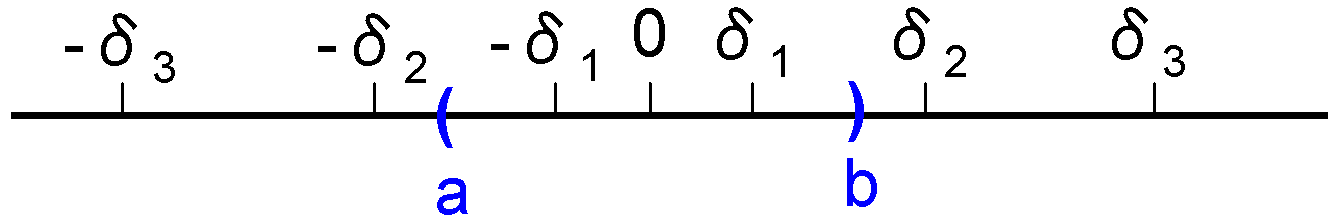
\includegraphics[height=0.4in,width=1.8in]{IncWiden.png} &
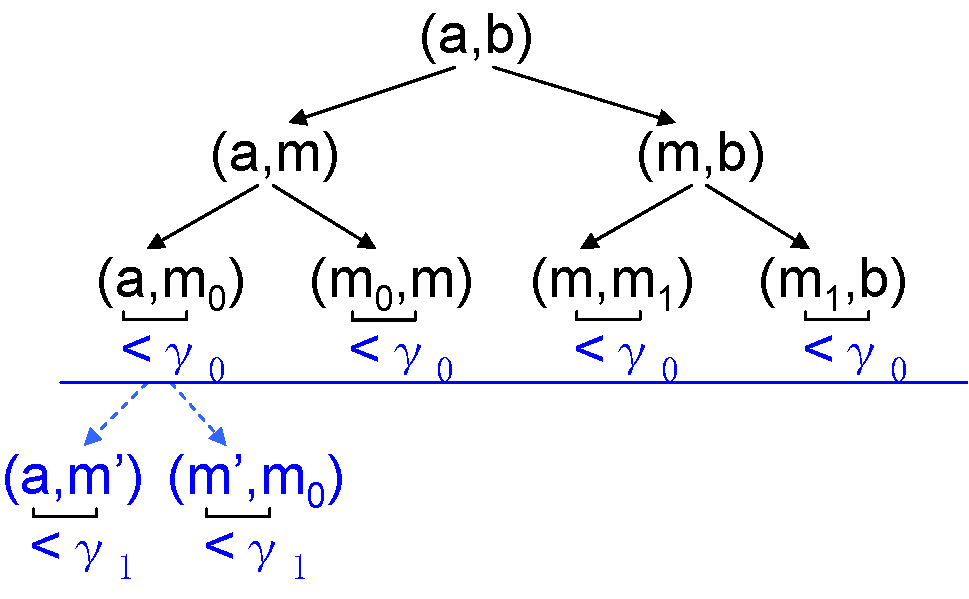
\includegraphics[height=1.2in,width=2in]{IncDeepen.png} \\
\mbox{(a) Incremenal widening} & \mbox{(b) Incremental Deepening} \\
\end{tabular}
\caption{Chebyshev approximation of $x^2$ and $x~|x|$}
\label{fig:incwid}
\end{minipage}
\end{figure}


\subsubsection*{Incremental deepening}

Starting with $F = \exists x_1 \in I_1 \cdots x_n \in I_n. \bigwedge \limits_{j=1}^m f_j > 0$, 
$I_1 \times \cdots \times I_n$ is decomposed into many boxes, 
and $F$ becomes the disjunction of existential formulae corrsponding to these boxes. 
{\bf raSAT} searches these boxes in depth-first manner, which may leads to exhaustive local search. 
To avoid it, {\bf raSAT} applies a threshold $\gamma$, such that no more decomposition will be 
applied when a box becomes smaller than $\gamma$. 
If neither SAT nor UNSAT is detected, {\bf raSAT} restarts with a smaller threshhold. 

Let $\gamma_0 > \gamma_1 > \cdots > 0$, and {\bf raSAT} incrementally deepens its search 
with these threshholds, i.e., starting with $\delta_0$, and if it fails, restart with $\delta_1$, 
and so on (Fig~\ref{fig:incwid} (b)). 



\subsection{SAT directed heuristics measure} \label{sec:SATheuristics}

With several hundred variables, we observe that an SMT solver works 
when either SAT, or UNSAT with small UNSAT core.
%
For the latter, we need an efficient heuristics to find an UNSAT core, which is left as future work. 
For the former, the keys are how to choose variables to decompose, and 
how to choose a box to explore. 
{\bf raSAT} chooses such a variable in two steps; first it selects a {\em test-UNSAT API}, and
then chooses a variable that appears in the API. 
We design SAT-directed heuristic measures based on the interval arithemtic ($O.T$). 

\sloppy
Let $F = \exists x_1 \in I_1 \cdots x_n \in I_n. \bigwedge \limits_{j=1}^m f_j > 0$ 
becomes ${\vee~( \exists x_1 \in I'_1 \cdots x_n \in I'_n. \bigwedge \limits_{j=1}^m f_j > 0)}$ 
after box decomposition. 
For $\exists x_1 \in I'_1 \cdots x_n \in I'_n. \bigwedge \limits_{j=1}^m f_j > 0$, 
if some $f_j > 0$ is UNSAT, the box $I'_1 \times \cdots \times I'_n$ is UNSAT. 
If every $f_j > 0$ is SAT, $F$ is SAT. 
Thus, if the box $I'_1 \times \cdots \times I'_n$ needs to be explore, it must contain 
a test-UNSAT API (thus IA-SAT). 

We denote the estimated range of $f_j$ for $x_1 \in I'_1 \cdots x_n \in I'_n$ with IA ($O.T$)
by $range(f_j, I'_1 \times \cdots \times I'_n)$. 
If an IA is an affine interval, 
it is in the form $[c_1,d_1]\epsilon_1 + \cdots + [c_n,d_n]\epsilon_n$, 
and we can obtain $range(f_j, I'_1 \times \cdots \times I'_n)$ by instantiating $\epsilon_i$ with $[-1,1]$ for $i \in \{1, \cdots, n\}$. 
We define 
\begin{itemize} 

\item {\em Sensitivity} of a variable $x_i$ in a test-UNSAT API $f_j > 0$ is $max(|c_i|, |d_i|)$. 
\item {\em SAT-likelihood} of an API $f_j > 0$ is $| I \cap (0,\infty) | / |I|$ where $I = range(f_j, I'_1 \times \cdots \times I'_n)$, and 
\item {\em SAT-likelihood} of a box $I'_1 \times \cdots \times I'_n$ is 
the least SAT-likelihood of test-UNSAT APIs. 
\end{itemize} 

\begin{example} \label{examp:SATlikelihood}
In Example~\ref{examp:sensitivity}, 
\begin{itemize}
\item sensitivity is estimated $1$ for $x$ and $2$ for $y$ by $AF_2$, and $3\frac{1}{4}$ for $x$ and 
$2$ for $y$. 
\item SAT-likelihood of $f$ is estimated $0.4= \frac{6}{9-(-6)}$ by $AF_2$ 
and $0.36 = \frac{4.5}{4.5-(-8)}$ by $CAI$. 
\end{itemize}
\end{example}


{\em SAT-likelihood} intends to estimate APIs how likely to be SAT. 
For choosing variables, {\bf raSAT} first choose a test-UNSAT API by SAT-likelihood. 
There are two choices, either {\em the largest} or {\em the least}. 
{\em Sensitivity} of a variable intends to estimate how a variable is influential to the value of an API. 
From a selected API by SAT-likelihood, {\bf raSAT} selects a variable with the largest sensitivity. 
This selection of variables are used for (1) {\em multiple test instances generation}, and 
(2) {\em decomposition}. 
For test generation, we will select multiple variables by repeating the selection. 

For choosing a box to explore, {\bf raSAT} chooses one which is more likely to be SAT. 
There are two choice, (1) a box with the largest SAT-likelihood, and 
(2) a box with the largest number of SAT (either IA-valid or test-SAT) APIs. 

\subsubsection*{Test case generation using variables sensitivity.}
\sloppy
The value of variables sensitivity can also be used to approximate how likely the value of a polynomial increases when the value of that variable increases. Consider the constraint $f = -x_{15}*x_8+x_{15}*x_2-x_{10}*x_{16}>0$. With ${x_2 \in [9.9, 10]}, {x_8 \in [0, 0.1]}, {x_{10} \in [0, 0.1]}, {x_{15} \in [0, 10]},$ and $ x_{16} \in [0, 10]$. The result of AF2 for $f$ is: $0.25 \epsilon_2 - 0.25 \epsilon_8 - 0.25 \epsilon_{10} + 49.5\epsilon_{15} - 0.25\epsilon_{16} + 0.75\epsilon_{+-} + 49.25$. The coefficient of $\epsilon_2$ is $0.25$ which is positive, then we expect that if $x_2$ increases, the value of $f$ is likely to increase.  As the result, the test case of $x_2$ is expected as high as possible in order to satisfy $f>0$. We will thus take the upper bound value of $x_2$, i.e. $10$, as a test case. Similarly, we take the test cases for other variables: $x_8=0, x_{10}=0, x_{15}=10, x_{16}=0$. With these test cases, we will have $f=100 > 0$.

\suppress{
I. Selecting API for testing:
  (1) Difficulty first by SAT-likelihood.   
  (2) Easy first by SAT-likelihood
  (10) Random.,
II. Selecting Variable:
  (8) With sensitivity
  (9) Without sensitivity - Random: 
III. Selecting box:
  (3) SAT-directed using IA-Testing.
  (4) UNSAT-directed using IA-Testing.
  (5) SAT-directed using SAT-likelihood
  (6) UNSAT-directed using SAT-likelihood
  (7) Random
}

\section{Experiments} \label{sec:experiment}

%\subsection{{\bf raSAT} Implementation} 
We implement \textbf{raSAT} loop as an SMT solver {\bf raSAT}, 
based on MiniSat 2.2 as a backend SAT solver. 
Various combinations of strategies of {\bf raSAT} (in Section~\ref{sec:strategy})
and random stategies are compared on {\em Zankl}, {\em Meti-Tarski} in NRA category 
and {\em AProVE} in NIA category from SMT-LIB. 
The best combination of choices are 
\begin{enumerate}
\item a test-UNSAT API by the least SAT-likelihood, 
\item a variable by the largest sensitivity, and 
\item a box by the largest SAT-likelihood, 
\end{enumerate} 
and sometimes a random choice of a test-UNSAT API (instead of the least SAT-likelihood) 
shows an equally good result. 
They are also compared with \textbf{Z3 4.3} and \textbf{iSAT3}, 
where the former is considered to be the state of the art (\cite{Jovanovic13}), and 
the latter is a popular ICP based tool. 
Note that our comparison is only on polynomial inequality. 
%Example~\ref{ex1} in Appendix~\ref{app:raSATexample} illustrates how {\bf raSAT} works. 
The experiments are on a system with Intel Xeon E5-2680v2 2.80GHz and 4 GB of RAM. 


\subsection{Benchmarks from SMT-LIB} \label{sec:expsmtlib}

In SMT-LIB\footnote{\tt http://www.smt-lib.org}, 
benchmark programs on non-linear real number arithmetic 
(QF\_NRA) are categorized into Meti-Tarski, Keymaera, Kissing, Hong, and Zankl families. 
Until SMT-COMP 2011, benchmarks are only Zankl family. 
In SMT-COMP 2012, other families have been added, and currently growing. 
General comparison among various existing tools on these benchmarks is summarized in 
Table.1 in \cite{Jovanovic13}, which shows Z3 4.3 is one of the strongest. 

From them, we extract problems of polynomial inequality only. %(not containing $''=''$). 
The brief statistics and explanation are as follows. 
\begin{itemize}
\item {\bf Zankl} has 151 inequalities among 166, taken from termination provers. 
A Problem may contain several hundred variables, an API may contain more than one hundred variable, 
and the number of APIs may be over thousands, though the maximum degree is up to $6$. 
\item {\bf Meti-Tarski} contains 5101 inequalities among 7713, taken from elementary physics.
They are mostly small problems, up to 8 varaibles (mostly up to 5 variables), and up to 20 APIs. 
\item {\bf Keymaera} contains 161 inequalities among 4442. 
\item {\bf Kissing} has 45 problems, all of which contains equality (mostly single equality). 
%They are taken from the cases of touching curves. 
\item {\bf Hong} has 20 inequalities among 20, tuned for QE-CAD and quite artificial. 
\end{itemize}


The setting of the experiments are
\begin{itemize}
\item For test data generation, raSAT chooses 10 variables (1 variable from each of 10 APIs with largest SAT-likelihood) and apply random 2-ticks, and single random test data is generated for each of the rest of variables.
\item For interval decomposition, raSAT applies the balanced decomposition.
\item For incremental widening, $\delta_0 = 10, \delta_1 = \infty$
\item For incremental deepening, $\gamma_i = 10^{-(i+1)}$ for $i \ge 0$.
\end{itemize}


\subsection{Experiments on strategy combinations} \label{sec:expstrategy}

We perform experiments only on inequalities of Zankl, and Meti-Tarski families. 
Table~\ref{tab:rasat-experiments} shows the experimental results of above mentioned combination. 
The timeout is set to 500s, and each time is the total of successful cases 
(either SAT or UNSAT). Our combinations of strategies are,

\medskip
{\centering
\begin{tabular}{l|l|l}
Selecting a test-UNSAT API~~ & Selecting a box (to explore): & 
Selcting a variable: \\  % (for testing and decomposition)
\hline

(1) Least SAT-likelihood. & 
(3) Largest number of SAT APIs.~~ & 
(8) Largest sensitibity. \\

(2) Largest SAT-likelihood. & 
(4) Least number of SAT APIs. & \\

& (5) Largest SAT-likelihood. & \\

& (6) Least SAT-likelihood. & \\

(10) Random. & (7) Random. & (9) Random. \\
\end{tabular}
}
\medskip

Note that (10)-(7)-(9) means all random selection. 
Generally speaking, the combination of (5) and (8) show the best results, 
though the choice of (1),(2), and (10) shows different behavior on benchmarks. 
We tentatively prefer (1) or (10), but it needs to be investigated further. 

\begin{table*}[t]
\centering
\adjustbox{max width=\columnwidth}{
\begin{tabular}{ | l | r | r | r | r  | r | r | r | r | r | r |r | r |}
\hline
    \multicolumn{1}{|l|}{Benchmark} & 
    \multicolumn{2}{c|}{(1)-(5)-(8)} & \multicolumn{2}{c|}{(1)-(5)-(9)} & 
    \multicolumn{2}{c|}{(1)-(6)-(8)} & \multicolumn{2}{c|}{(1)-(6)-(9)} &
    \multicolumn{2}{c|}{(10)-(5)-(8)} & \multicolumn{2}{c|}{(10)-(6)-(8)} 
\\
\hline
 Matrix-1 (SAT) & 20 & 132.72 (s) & 18 & 101.07 (s)& 15 & 1064.76 (s)& 14 & 562.19 (s)& \textbf{21} & 462.57 (s)& 18 & 788.46(s) 
\\
\hline
 Matrix-1 (UNSAT) & 2 & 0.01 (s)& 2 & 0.01 (s)&  2 & 0.01 (s)& 2 & 0.01 (s)& 2 & 0.01 (s)
& 2 & 0.01 (s)
\\
\hline
 Matrix-2,3,4,5 (SAT) & {\bf 10} & 632.37 (s)& 3 & 140.27 (s)& 1 & 3.46 (s)& 0 & 0.00 (s)& 5 & 943.08 (s)& 0 & 0.00 (s)
\\
\hline
 Matrix-2,3,4,5 (UNSAT) & 8 & 0.37 (s)& 8 & 0.39 (s)& 8 & 0.37 (s)& 8 & 0.38 (s)& 8 & 0.38 (s)& 8 & 0.38 (s)
\\
\hline
\hline
    \multicolumn{1}{|l|}{Benchmark} & 
    \multicolumn{2}{c|}{(2)-(5)-(8)} & \multicolumn{2}{c|}{(2)-(5)-(9)} & 
    \multicolumn{2}{c|}{(2)-(6)-(8)} & \multicolumn{2}{c|}{(2)-(6)-(9)} & 
    \multicolumn{2}{c|}{(2)-(7)-(8)} & \multicolumn{2}{c|}{(10)-(7)-(9)} \\
\hline
 Matrix-1 (SAT) & 20 & 163.47 (s) & 21 & 736.17 (s)& 19 & 953.97 (s)& 18 & 
1068.40 (s)& 19 & 799.79 (s)& 19 & 230.39 (s)
\\
\hline
 Matrix-1 (UNSAT) & 2 & 0.00(s) & 2 & 0.00 (s)& 2 & 0.00 (s)& 2 & 0.00 (s)& 2 & 0.00 (s)& 2 & 0.00 (s)
\\
\hline
 Matrix-2,3,4,5 (SAT) & 5 & 514.37 (s)& 1 & 350.84 (s)& 0 & 0.00 (s)& 0 & 0.00 (s)& 0 & 0.00 (s)& 1 & 13.43 (s)
\\
\hline
 Matrix-2,3,4,5 (UNSAT) & 8 & 0.43 (s)& 8 & 0.37 (s)& 8 & 0.40 (s)& 8 & 0.38 (s)& 8 & 0.37 (s)& 8 & 0.38 (s)
\\
\hline
\hline
    \multicolumn{1}{|l|}{Benchmark} & 
    \multicolumn{2}{c|}{(1)-(3)-(8)} & \multicolumn{2}{c|}{(1)-(4)-(8)} & 
    \multicolumn{2}{c|}{(2)-(3)-(8)} & \multicolumn{2}{c|}{(2)-(4)-(8)} & 
    \multicolumn{2}{c|}{(10)-(3)-(8)} & \multicolumn{2}{c|}{(10)-(4)-(8)} \\
\hline
 Matrix-1 (SAT) & 18 & 1438.47 (s) & 20 & 1537.9 (s)& 19 & 1100.60 (s)& 17 & 916.32 (s)& 17 & 87.78 (s)& 20 & 710.21 (s)
\\
\hline
 Matrix-1 (UNSAT) & 2 & 0.00 (s)& 2 & 0.00(s) & 2 & 0.00 (s)& 2 & 0.00 (s)& 2 & 0.00 (s)& 2 & 0.00 (s)
\\
\hline
 Matrix-2,3,4,5 (SAT) & 0 & 0.00 (s)& 1 & 33.17 (s)& 1 & 201.32 (s)& 2 & 328.03 (s)& 0 & 0.00 (s)& 1 & 20.94 (s)
\\
\hline
 Matrix-2,3,4,5 (UNSAT) & 8 & 0.36 (s)& 8 & 0.36 (s)& 8 & 0.34 (s)& 8 & 0.37 (s)& 8 & 0.37 (s)& 8 & 0.39 (s)
\\
\hline
\end{tabular}
}
\bigskip
\adjustbox{max width=\columnwidth}{
\begin{tabular}{ | l | r | r | r  | r | r | r | r | r |}
\hline
    \multicolumn{1}{|l|}{Benchmark} & 
    \multicolumn{2}{c|}{(1)-(5)-(8)} & \multicolumn{2}{c|}{(1)-(5)-(9)} & 
    \multicolumn{2}{c|}{(10)-(5)-(8)} & \multicolumn{2}{c|}{(10)-(7)-(9)} \\
\hline
    Meti-Tarski (SAT) & 3322 & 369.60 (s) & 3456 & 644.21 (s)& {\bf 3454} & 747.25 (s)& 3451 & 895.14 (s)
\\
\hline
    Meti-Tarski (UNSAT) & 1052 & 383.40 (s)& 1044 & 957.71 (s)& {\bf 1061} & 321.00 (s)& 1060 & 233.46 (s) 
\\
\hline
\end{tabular}
}
\medskip
\caption{Combnations of {\bf raSAT} strategies on NRA/Zankl,Meti-Tarski benchmark} 
\label{tab:rasat-experiments}
\end{table*}

Experiments in Table~\ref{tab:rasat-experiments} are performed 
with random generation ($k$-random tick) for the former and the blanced decomposition 
(dividing at the exact middle) for the latter. 

\subsection*{Experiments with test case generation using variables sensitivity}
From above section, we can see that the combination (1)-(5)-(8) shows the best performance on benchmarks. This section is going to examine the effectiveness of variables sensitivity in generation of test cases which is named as (11). Table~\ref{tab:test-sen} presents the result of the experiments on QF\_NRA/Zankl and QF\_NRA/Meti-tarski benchmarks, which show that this strategy made some improvements.

\begin{table}
\begin{center}
\begin{tabular}{ | l | r | r | r | r |}
\hline
    \multicolumn{1}{|l|}{Benchmark} & \multicolumn{2}{c|}{(1)-(5)-(8)} &
    \multicolumn{2}{c|}{(1)-(5)-(8)-(11)} \\
\hline
    Matrix-1 (SAT ) & 20 & 132.72 (s) & \textbf{25} & 414.99(s)
\\
\hline
    Matrix-1 (UNSAT) & 2 & 0.01(s) & 2 & 0.01(s)
\\
\hline
	Matrix-2,3,4,5 (SAT) & 10 & 632.37 (s) & \textbf{11} & 1264.77(s)
\\
\hline
    Matrix-2,3,4,5 (UNSAT) & 8 & 0.37(s) & 8 & 0.38(s)
\\ \hline
    Meti-Tarski (SAT) & 3322 & 369.60 (s) & 3322 & 369.60 (s)
\\
\hline
    Meti-Tarski (UNSAT) & 3322 & 369.60 (s) & 1052 & 383.40 (s)
\\
\hline
\end{tabular}
\end{center}
\caption{Effectiveness of variables sensitivity on test cases generation} 
\label{tab:test-sen}
\end{table}

\subsection{Comparison with other SMT solvers}

We compare {\bf raSAT} with other SMT solvers on NRA benchmarks, Zankl and Meti-Tarski. 
The timeout is $500s$. 
For {\bf iSAT3}, ranges of all variables are uniformly set to be in the range $[-1000, 1000]$
(otherwise, it often causes segmentation fault). 
Thus, UNSAT detection of {\bf iSAT3} means UNSAT in the range $[-1000, 1000]$, 
while that of {\bf raSAT}, \textbf{dReal} and {\bf Z3 4.3} means  UNSAT over $[-\infty, \infty]$. Another note is that if \textbf{dReal} concludes SAT, the constraint is $\delta$-SAT, which cannot imply the satisfiability of the constraint. For instances, with a number of UNSAT problems in Zankl, \textbf{dReal} still concludes SAT.

Among these SMT solvers, {\bf Z3 4.3} shows the best performance. 
However, if we closely observe, there are certain tendency. 
{\bf Z3 4.3} is very quick for small constraints, i.e., with 
short APIs (up to $5$) and a small number of variables (up to $10$). 
{\bf raSAT} shows comparable performance on SAT detection with 
longer APIs (larger than $5$) and a larger number of variables (more than $10$), 
and sometimes outforms for SAT detection on vary long constraints 
(APIs longer than $40$ and/or more than $20$ variables). 
Such examples appear in Zankl/matrix-3-all-*, matrix-4-all-*, and matrix-5-all-* 
(total 74 problems), and {\bf raSAT} solely solves 
\begin{itemize}
\item {\em matrix-3-all-2} (47 variables, 87 APIs, and max length of an API is 27), 
\item {\em matrix-3-all-5} (81 variables, 142 APIs, and max length of an API is 20), 
\item {\em matrix-4-all-3} (139 variables, 244 APIs, and max length of an API is 73), and 
\item {\em matrix-5-all-01} (132 variables, 276 APIs, and max length of an API is 47). 
\end{itemize}
Note that, for Zankl, when UNSAT is detected, it is detected very quickly. 
This is because SMT solvers detects UNSAT when they find small UNSAT cores, 
without tracing all APIs. However, for SAT detection with large problems, 
SMT solvers need to trace all problems. Thus, it takes much longer time. 

\begin{table*}[t]
\centering
\adjustbox{max width=\columnwidth}{
\begin{tabular}{ | l | r | r | r | r  | r | r | r | r | r | r |r | r | r | r | r | r |}
\hline
    \multicolumn{1}{|l|}{Benchmark} & 
    \multicolumn{4}{c|}{\bf raSAT} & \multicolumn{4}{c|}{\bf Z3 4.3} & \multicolumn{4}{c|}{\bf iSAT3} & \multicolumn{4}{c|}{\bf dReal}\\
\hline
    & \multicolumn{2}{c}{SAT} & \multicolumn{2}{|c}{UNSAT} & \multicolumn{2}{|c}{SAT} 
    & \multicolumn{2}{|c}{UNSAT} & \multicolumn{2}{|c}{SAT} & \multicolumn{2}{|c}{UNSAT} & \multicolumn{2}{|c}{$\delta-$SAT} & \multicolumn{2}{|c|}{UNSAT}\\
\hline
Zankl/matrix-1 (53) & 25 & 414.99 (s) & 2 & 0.01 (s) & \textbf{41} & 2.17 (s) & 12 & 0.00 (s) & 11 & 4.68 (s) & 3 & 0.00 (s) & 46 & 3573.43 (s) & 0 & 0.00 (s)\\
\hline
Zankl/matrix-2,3,4,5 (98) & 11 & 1264.77 (s) & 8 & 0.38 (s) & \textbf{13} & 1031.68 (s) & 11 & 0.57 (s) & 3 & 196.40 (s) & 12 & 8.06 (s) & 19& 2708.89 (s) & 0 & 0.00 (s) \\
\hline 
Meti-Tarski (5101) & 3322 & 369.60 (s) & 1052 & 383.40 (s) & 3528 & 51.22 (s) & 1568 & 78.56 (s) & 2916 & 811.53 (s) & 
1225 & 73.83 (s) & 3523 & 441.35 (s) & 1197 & 55.39 (s) \\
\hline
Keymaera (68) & 0 & 0.00 (s) & 16 & 0.06 (s) & 0 & 0.00 (s) & 68 & 0.36 (s) & 0 & 0.00 (s) & 
16 & 0.07 (s) & 8 & 0.18 (s) & 0 & 0.00 (s) \\
\hline
\end{tabular}
}
\medskip 
\caption{Comparison among SMT solvers over inequalities} \label{tab:comparison}
\end{table*}

\section{Extensions} \label{sec:eq}
\subsection{Extensions for Equality Handling}
\subsubsection*{Single Equation}
For solving polynomial constraints with single equality ($g=0$), we apply {\em Intermediate Value Theorem}. 
That is, if existing 2 test cases such that $g > 0$ and $g < 0$, then $g=0$ is SAT somewhere in between. 

\begin{lemma} \label{lemma:ivt}
For $F = \exists x_1 \in I_1 \cdots x_n \in I_n (\bigwedge \limits_{j}^m f_j > 0~\wedge~g = 0)$. Suppose decomposition creates a box $I = (l_1, h_1) \times \cdots \times (l_n, h_n)$ where $(l_i, h_i) \subseteq I_i$ for all $i \in \{1, \cdots, n\}$, such that $\bigwedge \limits_{j}^m f_j > 0$ is IA-VALID in the box. Let $(l_g, h_g) = range(g, I)$.
\begin{enumerate}[(i)]
\item If $l_g > 0$ or $h_g < 0$, then $F$ is UNSAT in the box. 
\item If there are two instances $\vec{t},\vec{t'}$ in the box with $g(\vec{t}) > 0$ and $g(\vec{t'}) < 0$, then F is SAT.
\end{enumerate}
\end{lemma}

\begin{proof}
\begin{enumerate}[(i)]
\item If $l_g > 0$ or $h_g < 0$, then $g=0$ cannot be satisfied in box $I$. As a result, $F$ is UNSAT in $I$. 
\item If there are two instances $\vec{t},\vec{t'}$ in the box with $g(\vec{t}) > 0$ and $g(\vec{t'}) < 0$, it is clear from the Intermediate Value Theorem that there exist one point $\vec{t_0}$ between $\vec{t}$ and $\vec{t'}$ such that $g(\vec{t_0}) = 0$. In addition, because $\bigwedge \limits_{j}^m f_j > 0$ is IA-VALID in $I$, $\vec{t_0}$ also satisfies $\bigwedge \limits_{j}^m f_j > 0$. As a result, $F$ is satisfiable with $\vec{t_0}$ as the SAT instance.
\end{enumerate}
\end{proof}
In the case that both (i) and (ii) do not occur, then \textbf{raSAT} continue by decomposition.
\begin{example}
Consider the constraint $\varphi = f(x, y) > 0 \wedge g(x, y) = 0$. Suppose we can find a box represented by $\Pi = x \in \langle a, b \rangle \wedge y \in \langle c, d \rangle$ such that $f(x, y) > 0$ is $\Pi^p_\mathbb{R}$-VALID (Figure~\ref{fig:single-equation}). In addition, inside that box, we can find two points $(u_1, v_1)$ and $(u_2, v_2)$ such that $g(u_1, v_1) > 0$ and $g(u_2, v_2) < 0$. By Lemma~\ref{lemma:ivt}, the constraint is satisfiable.
\end{example}
\begin{figure}[ht]
\centering
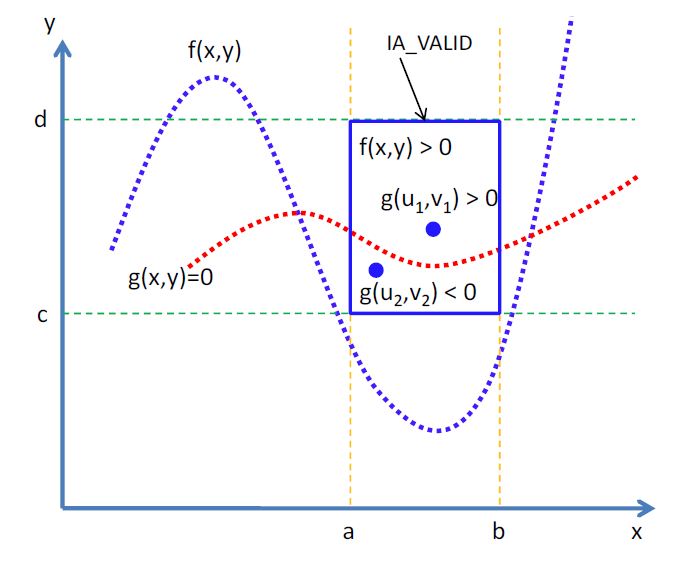
\includegraphics[scale=0.5]{singleEquation.png} 
\caption{Example on solving single equation using the Intermediate Value Theorem} 
\label{fig:single-equation} 
%\end{minipage}
\end{figure} 
{\bf raSAT} first tries to find a box of variables' intervals (by refinements) such that $\bigwedge \limits_{j}^m f_j > 0$ is VALID inside that box. Then it tries to find 2 instances for $g > 0$ and $g < 0$ by testing. 
Intermediate Value Theorem guarantees the existence of an SAT instance in between. 
Note that this method does not find an exact SAT instance. 
\subsubsection*{Multiple Equations}
The idea of using the Intermediate Value Theorem can also be used for solving multiple equations. 
Consider $m$ equations ($m \ge 1$): $\bigwedge \limits_{j=1}^m g_j = 0$ and an box $ I = {(l_1, h_1) \times \cdots (l_n, h_n)}$. If we can find a set ${\{V_1, \cdots, V_m\}}$ that satisfies the following properties, then we can conclude that $\bigwedge \limits_{j=1}^m g_j = 0$ is satisfiable in $I$.
\begin{itemize}
\item[$\bullet$] For all $j \in \{1, \cdots, m\}$, we have ${V_j \subseteq var(g_j)}$.
\item[$\bullet$] For all $j_1 \neq j_2\in \{1, \cdots, m\}$, we have $V_{j_1} \cap V_{j_2} = \emptyset$.
\item[$\bullet$] For all $j\in \{1, \cdots, m\}$, let $k_j = |V_j|$ and ${V_j = \{v_{jk} \; | \; 1 \le k \le k_j \}}$, then, there exist two combinations ${(x_{j1}, \cdots, x_{jk_j}) = (t_{j1}, \cdots, t_{jk_j})}$ and ${(x_{j1}, \cdots, x_{jk_j}) = (t'_{j1}, \cdots, t'_{jk_j})}$ where $t_{jk} \neq t'_{jk} \in (l_{jk}, h_{jk})$, $1 \le k \le k_j$ such that \[g_j(t_{j1}, \cdots, t_{jk_j}, \cdots, x_{jk}, \cdots) > 0\] and \[g_j(t'_{j1}, \cdots, t'_{jk_j}, \cdots, x_{jk}, \cdots) < 0\] for all values of $x_{jk}$ in $(l_{jk}, h_{jk})$ where $x_{jk} \in var(g_j) \setminus V_j$. We denote $ivt(g_j, V_j, I)$ to represent that the polynomial $g_j$ enjoy this property with respect to $V_j$ and $I$.
\end{itemize}
By the first two properties, this method restricts that the number of variables must be greater than or equal to the number of equations.

\begin{example}
Consider two equations $g_1(x, y)=0$ and $g_2(x, y) = 0$ (Figure~\ref{fig:multiple-equations}) which satisfy the above restriction on the number of variables, and the variable intervals are $x \in (c_1, d_1)$ and $y \in(d_2, c_2)$. Let $V_1 = \{x\}$ and $V_2 = \{y\}$, we have:
\[g_1(c_1, y) < 0\text{ and }g_1(d_1, y) < 0 \text{ for all } y \in \langle d_2, c_2 \rangle \text{; and }\]
\[g_2(x, d_2) > 0 \text{ and }g_2(x, c_2) < 0 \text{ for all } x \in \langle c_1, d_1 \rangle\]
Thus we can conclude that $g_1(x,y)=0 \wedge g_2(x,y)=0$ has a solution inside the box $(c_1, d_1) \times (d_2, c_2)$. This is because $ABCD$ creates a Jordan Curve and the continuous graph of $g_2$ connects one point in the interior to one point in the the exterior of that curve, so the graph of $g_2$ must intersects the curve somewhere.
\end{example}
\begin{figure}[ht]
\centering
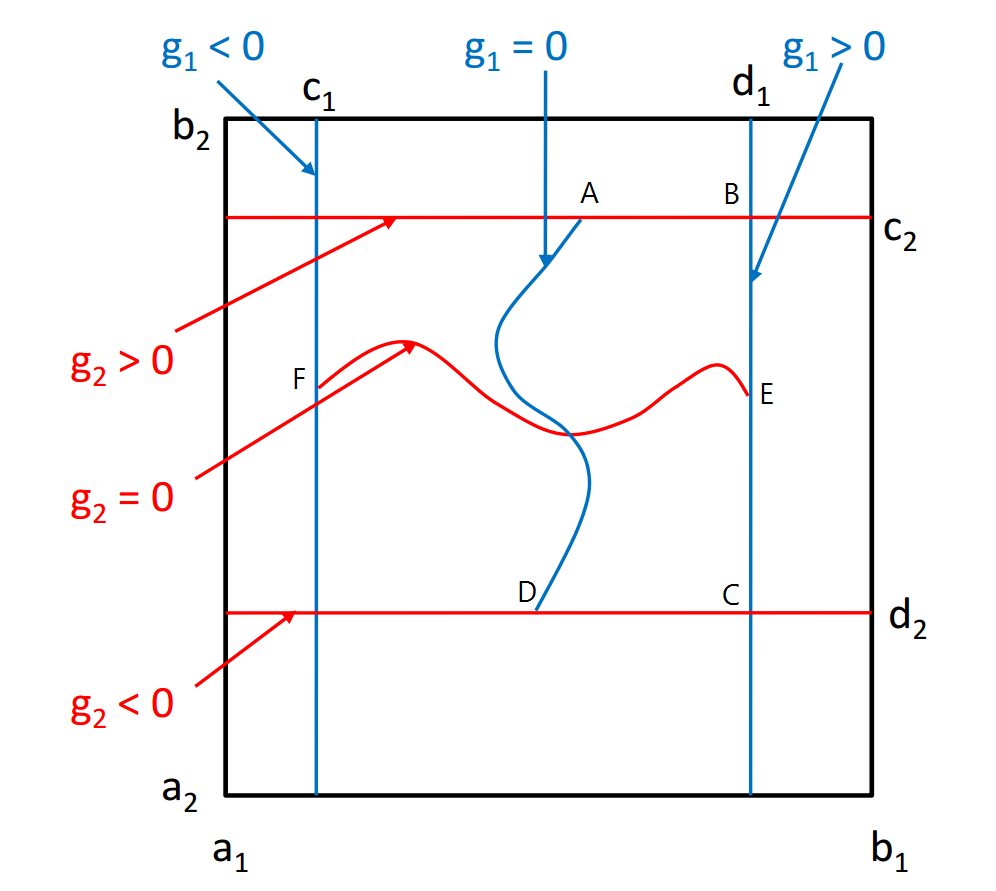
\includegraphics[scale=0.4]{multipleEquations.png} 
\caption{Example on solving single equation using the Intermediate Value Theorem} 
\label{fig:multiple-equations} 
%\end{minipage}
\end{figure}
Our current implementation of handling multiple equations is very naive
which is described in Algorithm~\ref{Al:multiple-equations}
because for each equality $g_j = 0$, \textbf{raSAT} checks every possible subsets of its variables as candidates for $V_j$. As a result, given the constraint $\bigwedge\limits_{j=1}^mg_j=0$, in the worst case \textbf{raSAT} will check $2^{|var(g_1)|}*\cdots*2^{|var(g_m)|}$ cases. As a future work, we may use variables' sensitivity to give priority on subsets of variables.
\begin{algorithm}
\begin{algorithmic}[1]
\Function{equationsProver}{$\bigwedge\limits_{i=j}^ng_i = 0, \Pi, V_0$}
\If {$j > n$} \Comment{All equations are checked}
	\State \Return SAT
\EndIf
\For {$V_j \in P(var(g_j))$} \Comment{$P(var(g_j))$ is the powerset of $var(g_j)$}
	\If {$V_j \cap V = \emptyset$ and $ivt(V', g_j, \Pi)$}
		\State $V_0 \gets V_0 \cup V'$
		\If {\Call{equationsProver}{$\bigwedge\limits_{i=j+1}^ng_i = 0, \Pi, V_0$} = SAT}
			\State \Return SAT
		\EndIf
	\EndIf
\EndFor
\State \Return UNSAT
\EndFunction
\State \Call{equationsProver}{$\bigwedge\limits_{i=1}^ng_i = 0, \Pi, \emptyset$}
\end{algorithmic}
\caption{Solving multiple equations $\bigwedge\limits_{i=1}^n g_i = 0$ with interval constraint ${\Pi = \bigwedge\limits_{v_i \in V} v_i \in \langle l_i, h_i \rangle}$}
\label{Al:multiple-equations}
\end{algorithm}

We also do experiments on constraints with equalities from QF\_NRA/Zankl and QF\_NRA/Meti-tarski. Table~\ref{tab:equations} 
\begin{table*}[t]
\centering
\adjustbox{max width=\columnwidth}{
\begin{tabular}{ | l | r | r | r | r  | r | r | r | r | r | r |r | r | r | r | r | r |}
\hline
    \multicolumn{1}{|l|}{Benchmark} & 
    \multicolumn{4}{c|}{\bf raSAT} & \multicolumn{4}{c|}{\bf Z3 4.3} & \multicolumn{4}{c|}{\bf iSAT3} & \multicolumn{4}{c|}{\bf dReal}\\
\hline
    & \multicolumn{2}{c}{SAT} & \multicolumn{2}{|c}{UNSAT} & \multicolumn{2}{|c}{SAT} 
    & \multicolumn{2}{|c}{UNSAT} & \multicolumn{2}{|c}{SAT} & \multicolumn{2}{|c}{UNSAT} & \multicolumn{2}{|c}{$\delta-$SAT} & \multicolumn{2}{|c|}{UNSAT}\\
\hline
Zankl (15) & \textbf{11} & 0.07 (s) & \textbf{4} & 0.17 (s) & \textbf{11} & 0.17 (s) & \textbf{4} & 0.02 (s) & 0 & 0.00 (s) & \textbf{4} & 0.05 (s) & 11 & 0.06 (s) & \textbf{4} & 0.02(s)\\
\hline
Meti-Tarski (3528/1573) & 3322 & 369.60 (s) & 1052 & 383.40 (s) & 1497 & 21.00 (s) & 1115 & 74.19 (s) & 1 & 0.28 (s) & 
1075 & 22.6 (s) & 1497 & 72.85 (s) & 943 & 21.40 (s) \\
\hline
Keymaera (612) & 0 & 0.00 (s)& 312 & 66.63 (s) & 0 & 0.00 (s) & \textbf{610} & 2.92 (s) & 0 & 0.00 (s) & 226 & 1.63 (s) & 13& 4.03 (s) & 318 & 1.96 (s) \\
\hline 
\end{tabular}
}
\medskip 
\caption{Comparison among SMT solvers over equalities} \label{tab:equations}
\end{table*}

\subsection{Extension for Polynomial Constraints Over Integers} \label{sec:NIA}

{\bf raSAT} loop is easily modified to NIA (nonlinear arithmetic over integers) from NRA, 
by setting $\gamma_0 = 1$ in incremental deepening in Section~\ref{sec:incsearch} 
and restrcting testdata generation on intergers. 
We also compare {\bf raSAT} (combination (1)-(5)-(8)-(11) with {\bf Z3 4.3} on NIA/AProVE benchmark. 
{\bf AProVE} consists of 6850 inequalities and 1979 equalities. 
Some has several hundred variables, but each API has few variables (mostly just 2 variables). Note that the use of the Intermediate Value Theorem cannot be applied for NIA constraints because the polynomials are not continuous. However, Interval Arithmetics can conclude UNSAT of QF\_NIA benchmarks because UNSAT over real numbers simply implies UNSAT over integer numbers. For SAT benchmarks (both inequalities and equalities), \textbf{raSAT} concludes satisfiability only by testing.

The results are presented in Table~\ref{tab:aprove}
\suppress{
\begin{itemize}
\item {\bf raSAT} detects 6773 SAT in 90.22s, and 2 UNSAT in 378.04s. 
\item {\bf Z3 4.3} detects 6784 SAT in 97.70s, and 36 UNSAT in 32.08s. 
\end{itemize}
}
where the timeout is $500s$. 
{\bf raSAT} does not detect unsatisfiability well since UNSAT problems have quite large coefficients
which lead exhaustive search on quite large area.

\begin{table*}[t]
\centering
\begin{tabular}{ | l | r | r | r | r  | r | r | r | r |}
\hline
    \multicolumn{1}{|l|}{Benchmark} & 
    \multicolumn{4}{c|}{\bf raSAT} & \multicolumn{4}{c|}{\bf Z3 4.3}\\
\hline
    & \multicolumn{2}{c}{SAT} & \multicolumn{2}{|c}{UNSAT} 
    & \multicolumn{2}{|c}{SAT} & \multicolumn{2}{|c|}{UNSAT} \\
\hline
inequalities (6850) & \textbf{6784} & 65.60 (s) & 0 & 0.00 (s) & \textbf{6784} & 97.77 (s) & \textbf{36} & 32.46 (s) 
\\
\hline
equalities (1979) & 891 & 33721.37 (s) & 16 & 27.34 (s) & \textbf{900} & 1951.01(s) & \textbf{250} & 3104.74(s) 
\\
\hline
\end{tabular}
\medskip 
\caption{Comparison on NIA/AProVE} \label{tab:aprove}
\end{table*}

%%%%%%%%%%%%%%%%%
\suppress{
\section{Equality handling} \label{sec:equality}

\subsection{Greater-than-or-Equal Handling} \label{sec:geq}

{\bf raSAT} loop is designed to solve polynomial inequality. 
There are several ways to extend to handle equality, in which our idea shares similarity with 
dReal~\cite{dRealCADE13,dRealLICS12}. 

\begin{definition} \label{def:strict_unsat}
$\bigwedge \limits_{j} f_j \geq 0$ is 
{\em strict-SAT} (resp. {\em strict-UNSAT}) 
if $\bigwedge \limits_{j} f_j > \delta_j$ is SAT 
(resp. $\bigwedge \limits_{j} f_j > -\delta_j$ is UNSAT) for some $\delta_j >0$.
\end{definition}

\begin{lemma} \label{lem:strict_sat}
If $\bigwedge \limits_{j} f_j \geq 0$ is {\em strict-SAT} (resp. {\em strict-UNSAT}), 
it is SAT (resp. UNSAT).
\end{lemma}

Note that netiher strict-SAT nor strict-UNSAT (i.e., kissing situation), 
%if $\bigwedge \limits_{j} f_j \geq 0$ is SAT but $\bigwedge \limits_{j} f_j > 0$ is UNSAT 
Lemma~\ref{lem:strict_sat} cannot conclude anything, and \textbf{raSAT} says {\em unknown}. 
%In implementation of \textbf{raSAT}, when $\geq$ appears, exploration of IA-SAT 
%(resp. IA-UNSAT) is reduced to that of IA-strict-SAT (resp. IA-strict-UNSAT). 


\subsection{SAT on Equality by Intermediate Value Theorem} \label{sec:eq}
For solving polynomial constraints with single equality ($g=0$), we apply {\em Intermediate Value Theorem}. 
That is, if existing 2 test cases such that $g > 0$ and $g < 0$, then $g=0$ is SAT somewhere in between, 
as in Fig.~\ref{fig:ivt}. 

\begin{lemma} \label{lemma:ivt}
For $F = \exists x_1 \in (a_1,b_1) \wedge \cdots \wedge x_n \in (a_n,b_n). 
\bigwedge \limits_{j}^m f_j > 0~\wedge~g = 0$, $F$ is SAT, if 
there is a box $(l_1, h_1) \times \cdots \times (l_n,h_n)$ with $ (l_i,h_i) \subseteq (a_i,b_i)$ 
such that 
\begin{enumerate}[(i)]
\item $\bigwedge \limits_{j}^m f_j > 0$ is IA-VALID in the box, and 
\item there are two instances $\vec{t},\vec{t'}$ in the box with $g(\vec{t}) > 0$ and $g(\vec{t'}) < 0$.
\end{enumerate}
\end{lemma}

{\bf raSAT} first tries to find an IA-VALID box for $\bigwedge \limits_{j}^m f_j > 0$ by refinements. 
If such a box is found, it tries to find 2 instances for $g > 0$ and $g < 0$ by testing. 
Intermediate Value Theorem guarantees the existence of an SAT instance in between. 
Note that this method works for single equality and does not find an exact SAT instance. 
If multiple equalities do not share variables each other, we can apply Intermediate Value Theorem 
repeatedly to decide SAT. In Zankl benchmarks in SMT-lib, there are 15 gen-**.smt2 that contain equality
(among 166 problems), and each of them satisty this condition. 


 
\suppress{
In Table \ref{tab:eqexp} we show preliminary experiment for 15 problems that contain polynomial equalities in Zankl family. \textbf{raSAT} works well for these SAT problems and it can detect all SAT problems (11 among 15). At the current implementation, raSAT reports \emph{unknown} for UNSAT problems. The first 4 columns indicate \emph{name of problems}, \emph{the number of variables}, \emph{the number of polynomial equalities} and \emph{the number of inequalities}  in each problem, respectively. The last 2 columns show comparison results of \textbf{Z3 4.3} and \textbf{raSAT}.
\begin{table}
\centering
\scalebox{1.0}{
\begin{tabular}[b]{|c|c|c|c|c|c|c|c|}
\hline
%\multirow{2}{*}{Problem} & {No.} & {No.} & {No.}&
{Problem} & {No.} & {No.} & {No.}&
\multicolumn{2}{c|}{\textbf{Z3 4.3} (15/15)} &\multicolumn{2}{c|}{\textbf{raSAT} (11/15)}\\
\cline{5-8}
Name & Variables& Equalities& Inequalities&{Result} & {Time(s)}&{Result} & {Time(s)}\\
\hline
gen-03 & 1 & 1 & 0& SAT &0.01 & SAT &0.015\\
\hline
gen-04 & 1 & 1 & 0& SAT &0.01 & SAT &0.015\\
\hline
gen-05 & 2 & 2 & 0& SAT &0.01 & SAT &0.046\\
\hline
gen-06 & 2 & 2 & 1& SAT &0.01 & SAT &0.062\\
\hline
gen-07 & 2 & 2 & 0& SAT &0.01 & SAT &0.062\\
\hline
gen-08 & 2 & 2 & 1& SAT &0.01 & SAT &0.062\\
\hline
gen-09 & 2 & 2 & 1& SAT &0.03 & SAT &0.062\\
\hline
gen-10 & 1 & 1 & 0& SAT &0.02 & SAT &0.031\\
\hline
gen-13 & 1 & 1 & 0& UNSAT &0.05 & unknown &0.015\\
\hline
gen-14 & 1 & 1 & 0& UNSAT &0.01 & unknown &0.015\\
\hline
gen-15 & 2 & 3 & 0& UNSAT &0.01 & unknown &0.015\\
\hline
gen-16 & 2 & 2 & 1& SAT &0.01 & SAT &0.062\\
\hline
gen-17 & 2 & 3 & 0& UNSAT &0.01 & unknown &0.031\\
\hline
gen-18 & 2 & 2 & 1& SAT &0.01 & SAT &0.078\\
\hline
gen-19 & 2 & 2 & 1& SAT &0.05 & SAT &0.046\\
\hline
\end{tabular}
}
\caption{Experimental results for 15 equality problems of Zankl family}
\label{tab:eqexp}
\end{table}

We also apply the same idea for multiple equalities $\bigwedge \limits_{i} g_i = 0$ such that $Var(g_k) \cap Var(g_{k'}) = \emptyset$ where $Var(g_k)$ is denoted for the set of variables in the polynomial $g_k$. In the next section we will present idea for solving general cases of multiple equalities.
}

}
%%%%%%%%%%%%%%%%%%%%%%%%%%%%%



\section{Conclusion} \label{sec:conclusion and Future Work}


This paper presented {\bf raSAT} loop, which extends ICP with testing to accelerate
SAT detection and implemented as an SMT solver \textbf{raSAT}. With experiments on benchmarks from QF NRA category of SMT-lib, we found two heuristic measures SAT-likelihood and sensitivity, which lead effective strategy combination for SAT detection. 
%
\suppress{
\subsection{Observation and Discussion} 

From experimental results in Section~\ref{sec:experiments} and~\ref{sec:expsmtlib}, 
we observe the followings. 
\begin{itemize}
\item The degree of polynomials will not affect much. 
\item The number of variables are matters, but also for Z3 4.3. 
The experimental results do not show exponential growth, and we expect 
the strategy of selection of an API in which related intervals are decomposed
seems effective in practice. By observing Zankl examples, we think the maximum 
number of variables of each API seems a dominant factor. 
\item Effects of the number of APIs are not clear at the moment. In simple benchmarks, 
{\bf raSAT} is faster than Z3 4.3, however we admit that we have set small degree $n=6$
for each API. 
\end{itemize}

For instance, {\em matrix-2-all-5,8,11,12} in Zankl 
contain a long monomial (e.g., $60$) with the max degree $6$, and 
relatively many variables (e.g., $14$), which cannot be solved by Z3 4.3, but 
{\bf raSAT} does. 
As a general feeling, if an API contains more than $30 \sim 40$ variables, 
{\bf raSAT} seems saturating. 
We expect that, adding to a strategy to select an API (Section~\ref{sec:intervaldecomp}), 
we need a strategy to select variables in the focus. We expect this can be designed 
with sensitivity (Example~\ref{examp:sensitivity}) and would work in practice. 
Note that sensitivity can be used only with noise symbols in Affine intervals. 
Thus, iSAT and RSOLVER cannot use this strategy, though they are based on IA, too. 

\subsection{Future Work}
}
%
{\bf raSAT} still remains in naive proto-type status, and 
there are lots of future work. 

\medskip \noindent 
{\bf UNSAT core}. Currently, \textbf{raSAT} focuses on SAT detection. For
UNSAT detection, the target is to find a small UNSAT core in a large problem.


\medskip \noindent 
{\bf Equality handling}. 
Section~\ref{sec:eq} shows equality handling where UNSAT constraints can be completely solved by ICP (with the assumption of bounded intervals). The Intermediate Value Theorem can be used to show satisfiability with restrictions on variables of polynomials. Moreover, the use of this theorem is not a complete in showing satisfiability. As a future work, we will apply Groebner basis.

\medskip \noindent 
{\bf Further strategy refiment}. 
Currently, raSAT uses only information from
O.T (interval arithmetic).We are planning to refine strategies such that previous
O.T and U.T results mutually guide to each other. For instance, test generation
and a box decomposition can be more focused.1


%%%
\suppress{
\subsubsection{Extension of {\bf raSAT} loop}
\begin{itemize}
\item {\bf Equality handling}: currently, {\bf raSAT} loop can handle only inequalities. 
Before applying ideal based technique, such as {\em Gr{\"o}bner basis}, 
we are planning to implement a non-constructive detection of equality 
by {\em intermediate value theorem}. 

\suppress{
\item{\textbf{Polynomial equality by Intermediate value theorem}:} 
Consider 
\begin{center}
$(x_1 \in (a_1,b_1) \wedge \cdots \wedge x_n \in (a_n,b_n))~\bigwedge 
\limits_{j}^m f_j(x_1,\cdots,x_n) > 0~\wedge~g(x_1,\cdots, x_n) = 0.$
\end{center}
SAT can be proved by two steps. First, find a box of the product of 
$(l_{ik},h_{ik}) \subseteq (l_i,h_i)$ (by interval arithmetic) such that 
\begin{center}
$\forall x_1 \in (l_{1k},h_{1k}) \cdots x_n \in (l_{nk},h_{nk}).~\bigwedge 
 \limits_{j}^m f_j(x_1,\cdots,x_n) > 0$~~~~(IA-VALID) 
\end{center}
and find two instances (by testing) in the box with $g(a_1,\cdots,a_n) > 0$ 
and $g(b_1,\cdots,b_n) < 0$. By Intermediate value theorem, we can conclude 
$\exists x_1 \in (l_1,h_1) \cdots x_n \in (l_n,h_n).~g(x_1,\cdots, x_n) = 0$. 
}

\item \textbf{Solving polynomial constraints on integers}: 
In integer domain, the number of test data is finite if interval constraints are bounded. 
Then, Test-UNSAT implies UNSAT if all possible test data are generated. 
A tight interaction between testing and interval decomposition could be investigated.
Mixed integers are also challenging. 
\end{itemize}


\subsubsection{\textbf{raSAT} Development}

\begin{itemize}
\item \textbf{Avoiding local optimal}: 
we borrow an idea of \emph{restart} in MiniSAT for escaping from hopeless local search 
(i.e., solution set is not dense or empty). 
\emph{Heuristics} would be, after a deep interval decomposition of 
a box and Test-UNSAT are reported, backtrack occurs to choose a randomly selected box. 

\item \textbf{Separation of linear constraints}: 
Many benchmarks contain linear constraints. Current implementation does not have 
any tuning, but {\bf raSAT} loop only. 
Practically, separating linear and non-linear constraints and solving them 
in a coordinated way between Presbuger arithmetic and {\bf raSAT} would improve. 
During this separation, variables of intersecting linear constraints would be candidates 
for interval decompositions. 

\item \textbf{Incremental DPLL}: For interactions with the SAT solver, 
we currently apply the very lazy theory learning. Combination with 
\emph{eager} theory propagation would improve, in which we can propagate 
a conflict from a partial truth assignment instead of waiting 
for a full truth assignment obtained by SAT solver.
\end{itemize}
}
%%

%%
\suppress{
\subsection{Applications}
\begin{itemize}
\item \textbf{Checking overflow and roundoff error}: In the computers, the real numbers are represented by finite numbers (i.e., floating point numbers, fixed point numbers). Due to finite representation, the over-flow and roundoff errors (OREs) \cite{ngocsefm, ngocase} may occur. The OREs will be propagated through computations of the program. Further, the computations themselves also cause OREs because the arithmetic needs to round the result to fit the number format. Besides, OREs are also affected by types of statements, i.e., branch, loop, assignment statements.
By symbolic execution, ORE constraints are propagated from a program and ORE problems are reduced to problems of solving ORE constraints for verifying whether OREs occur. 
%For solving ORE constraint, combination of the new form of affine arithmetic ($CAI_1$) and \emph{sensitivity} (i.e., high degrees, )

\item \textbf{Loop invariant generation}: The problem of linear invariant generation is often reduced to the problem of non-linear constraint solving. 
Since Farkas's Lemma \cite{Colon03} uses the product of matrices with polynomial constraint solving, we can extend the target for non-linear invariant generation.
%Based on Farkas' Lemma \cite{Colon03}, non-linear constraints on coefficients of the target linear invariant are generated and a satisfiable instance of these constraints is a candidate of the linear invariant. 
\end{itemize}
}
%%


%\balance
\bibliographystyle{splncs}
\bibliography{generic}


\end{document}


